\documentclass{book}
\usepackage{graphicx}                              %for PNG images (pdflatex)
\usepackage[linkbordercolor={1.0 1.0 0.0}]{hyperref} %for \url tag
\usepackage{color}                                 %for defining custom colors
\usepackage{framed}                                %for shaded and framed paragraphs
\usepackage{textcomp}                              %for various symbols, e.g. Registered Mark
\usepackage{geometry}                              %for defining page size
\usepackage{longtable}                             %for breaking tables
\usepackage{trackchanges}
%
\geometry{verbose,a4paper,tmargin=2.5cm,bmargin=2.5cm,lmargin=2.5cm,rmargin=2CM}
\hypersetup{
  pdfauthor = {Zsombor Nagy},
  pdftitle = {Documentation of the ARC storage system},
  pdfsubject = {Paper subject},
  pdfkeywords = {Paper,keyword,comma-separated},
  pdfcreator = {PDFLaTeX with hyperref package},
  pdfproducer = {PDFLaTeX}
}
%
\bibliographystyle{IEEEtran}                       %a nice bibliography style
%
\def\efill{\hfill\nopagebreak}%
\hyphenation{Nordu-Grid}
\setlength{\parindent}{0cm}
\setlength{\FrameRule}{1pt}
\setlength{\FrameSep}{8pt}
\addtolength{\parskip}{5pt}
\renewcommand{\thefootnote}{\fnsymbol{footnote}}
\renewcommand{\arraystretch}{1.3}
\newcommand{\dothis}{\colorbox{shadecolor}}
\newcommand{\ngdl}{\url{http://ftp.nordugrid.org/download}~}
\definecolor{shadecolor}{rgb}{1,1,0.6}
\definecolor{salmon}{rgb}{1,0.9,1}
\definecolor{bordeaux}{rgb}{0.75,0.,0.}
\definecolor{cyan}{rgb}{0,1,1}
%
%----- DON'T CHANGE HEADER MATTER
\hyphenation{preserve-Original}
\begin{document}
\def\today{\number\day/\number\month/\number\year}

\begin{titlepage}

\begin{tabular}{rl}
\resizebox*{3cm}{!}{
\includegraphics{ng-logo.png}}
&\parbox[b]{2cm}{\textbf \it {\hspace*{-1.5cm}NORDUGRID\vspace*{0.5cm}}}
\end{tabular}

\hrulefill

%-------- Change this to NORDUGRID-XXXXXXX-NN

{\raggedleft NORDUGRID-TECH-17\par}

{\raggedleft \today\par}

\vspace*{2cm}

%%%%---- The title ----
{\centering \textsc{\Large Chelonia - Self-healing distributed storage system}\Large \par}
\vspace*{0.5cm}
    
%%%%---- A subtitle, if necessary ----
{\centering \textit{\large Documentation and developer's guide}\large \par}
    
\vspace*{1.5cm}
%%%%---- A list of authors ----
    {\centering \large Zsombor Nagy\footnote{zsombor@niif.hu} \large \par}
    {\centering \large Jon Nilsen\footnote{j.k.nilsen@usit.uio.no} \large \par}
    {\centering \large Salman Zubair Toor \footnote{salman.toor@it.uu.se} \large \par}
\end{titlepage}

\tableofcontents                          %Comment if use article style
\newpage

\renewcommand{\thefootnote}{\arabic{footnote}}


\chapter{Design Overview} % (fold)
\label{cha:overview}


Chelonia is a distributed system for storing replicated \emph{file}s on several file storage nodes and managing them in a global namespace.  The files can be grouped into \emph{collection}s (a concept very similar to directories in the common file systems). A collection can contain sub-collections and sub-sub-collections in any depth. There is a dedicated \emph{root collection} to gather all collections to the global namespace. This hierarchy of collections and files can be referenced using \emph{Logical Name}s (\emph{LN}'s). The users can use this global namespace as if they were using a local filesystem. Files can be transfered by several different transfer protocols. The client side tools hide this from the user. The replicas of the files are stored on different storage nodes. A storage node here is a network-accessible computer having storage space to share, and a running storage element service (e.g.~HTTP(S), FTP(S), GridFTP, ByteIO\footnote{OGSA ByteIO Working Group (BYTEIO-WG), \url{https://forge.gridforum.org/projects/byteio-wg/}}, etc.). On each storage node a Chelonia service is needed to be installed to manage and integrate it into the system. The client side provides access to third-party storage solutions through the namespace of Chelonia. The main services of the storage system are the following (see Figure~\ref{fig:services}):
\begin{itemize}
    \item the \textbf{A-Hash} service, which is a replicated database which is used by the Librarian to store metadata;
    \item the \textbf{Librarian} service, which handles the metadata and hierarchy of collections and files, the location of replicas, and health data of the Shepherd services, using the A-Hash as database;
    \item the \textbf{Bartender} service, which provides a high-level interface for the users and for other services;
    \item the \textbf{Shepherd} service, which manages storage element services, and provides a simple interface for storing files on storage nodes.
\end{itemize}

\begin{figure}[ht]
\centering{{\scalebox{0.8}{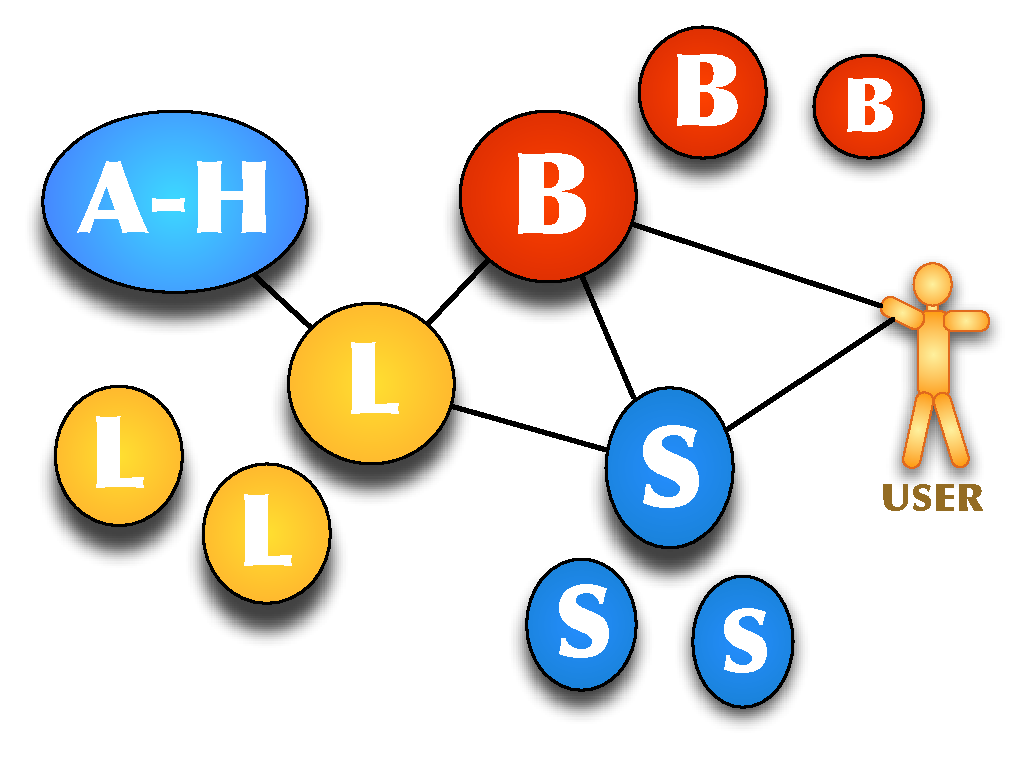
\includegraphics{arc-storage-services.pdf}}}
\caption{\label{fig:services} The components of Chelonia: the \textbf{A-H}ash service, the \textbf{L}ibrarian service, the \textbf{B}artender service and the \textbf{S}hepherd service.}}
\end{figure}

\section{Files and collections} % (fold)
\label{sec:files_and_collections}

The storage system is capable of storing files which can be grouped in collections and sub-collections, etc.
Every file and collection has a unique ID in the system called the \emph{GUID}. Compared to the well-known structure of local file systems, these GUID's are very similar to the concept of \emph{inode}s. And as a directory on a local filesystem is basically just a list of name and inode pairs, a collection in Chelonia is just a list of name and GUID pairs. There is a dedicated collection which is the \emph{root collection}. This makes the namespace of Chelonia a hierarchical namespace where you can start at the root collection, and go to sub-collections and sub-sub-collections to get to a file. This path is called the \emph{Logical Name} (LN). For example if there is a sub-collection called \verb!saturn! in the root collection, and there is a file called \verb!rings! in this sub-collection, then the LN of this file is \verb!/saturn/rings!.

In addition to the Logical Names we can refer to a file or collection simply by its GUID, or we can use GUID's and Logical Names together, as seen in Figure~\ref{fig:namespace}.

The full syntax of Logical Names is \verb#/[path]# or \verb#<GUID>[/<path>]# where [...] indicates optional parts.

\begin{figure}[ht]
\centering{{\scalebox{0.7}{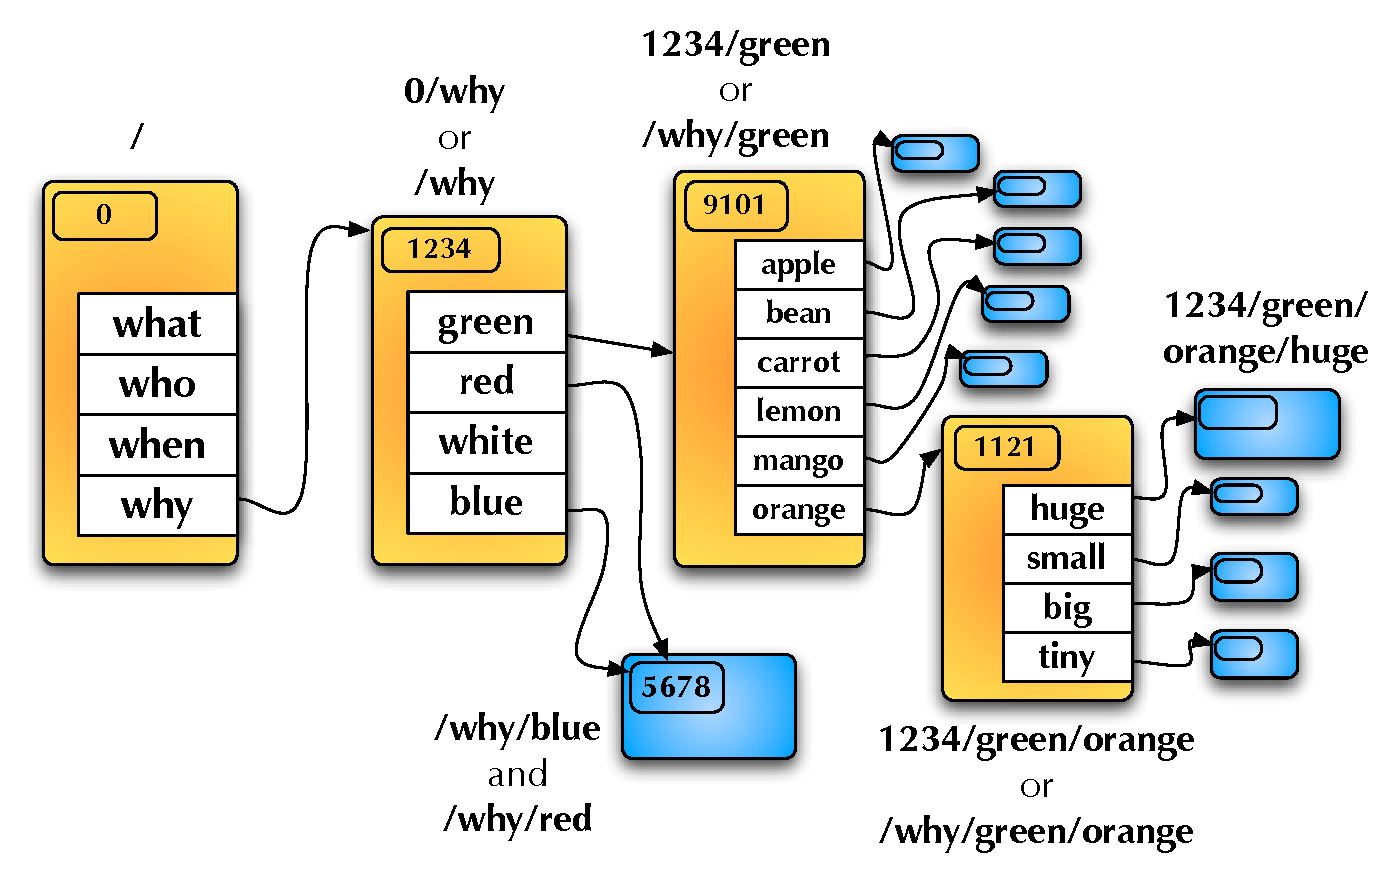
\includegraphics{arc-storage-namespace.pdf}}}
\caption{\label{fig:namespace}Example of the hierarchy of the global namespace} }
\end{figure}

An example of the hierarchy of the global namespace is shown in Figure~\ref{fig:namespace}: if we have a collection with GUID \verb#1234#, and there is a collection called \verb#green# in it, and in \verb#green# there is another collection called \verb#orange#, and in \verb#orange# there is a file called \verb#huge#, then we can refer to this file with the Logical Name \verb#1234/green/orange/huge#, which means that from the collection called \verb!1234! we have to follow along the path: \verb!green!, \verb!orange!, \verb!huge!.

There is a dedicated root collection (which has the GUID \verb#0#), and if a LN starts without a GUID prefix, it is implicitly prefixed with the GUID of the root collection, e.g.~\verb#/why/blue# means \verb#0/why/blue#. If a user wants to find the file called \verb#/why/blue#, the system knows where to start the search: the GUID of the root collection. The root collection knows the GUID of \verb#why#, and the (sub-)collection \verb#why# knows the GUID of \verb#blue#. If the GUID of this file is \verb#5678#, and somebody makes another entry in collection \verb#/why# (= \verb#0/why#) with name \verb#red# and GUID \verb#5678#, then the \verb#/why/red# LN points to the same file as \verb#/why/blue#, a concept very similar to a hardlink in a regular local (POSIX-like) file system.

% section files_and_collections (end)

\section{Storage nodes and replicas} % (fold)
\label{sec:storage_nodes_and_replicas}

The collections in Chelonia are logical entities. The content of a collection is stored as metadata of the collection, which means that a collection actually has no physical data. A file, however, has both metadata and real physical data (the actual content of the file). The metadata of a file is stored in the same database where the collections are stored, but the physical data of a file is stored on storage nodes as multiple replicated copies.

A storage node consists of two things: a storage element service which is capable of storing and serving files through a specific protocol (e.g. a web server, an FTP server, a GridFTP server, etc.) and a Shepherd service which provides a simple interface to access the storage node, and which can initiate and manage file transfers through the storage element service. The Shepherd has different backends for the supported storage element services which made it possible to communicate with them.

A logical file, which are part of the hierarchical namespace, has a GUID and other metadata, and one or more physical replicas. The physical replicas are stored on separate storage nodes. In order to connect the logical file to its replicas, the system needs to have global pointers. Each storage node has a URL and each replica has a unique ID within the storage node called \emph{referenceID}, the URL and the referenceID together is called a \emph{Location}, a Location unambiguously points to one specific replica. To connect the logical files to the physical ones, each logical file has a list of Locations.

The user can specify how many replicas are required for each file. The storage nodes periodically check the number of replicas for each file they store, and automatically creates new replicas if there are fewer than required, and removes replicas if there are more. (Currently if a storage node stores a great amount of files, then the checking period could be longer.)

The file replicas can be in the following states: the replica can be valid and alive or just in the process of creation or it may be corrupt or a whole storage node may be offline. This state is always stored as metadata of the given replica. For each file there is a checksum calculated, and this checksum is used to detect if a replica gets corrupted. If a storage node (more precisely: the Shepherd service on the storage node) detects that a file is invalid, it reports this so the metadata will be in sync with the real state. And the storage nodes sends heartbeat messages periodically, and if a storage node goes offline, the missing heartbeat also triggers the modification of metadata. 

% section storage_nodes_and_replicas (end)

\section{The A-Hash} % (fold)
\label{sec:the_a_hash}

The A-Hash is the metadata store of the storage system. The A-Hash may be deployed as either a centralized or a replicated service. It consistently stores `objects' which contain property-value pairs organized in sections. All metadata about files and collections in the storage system are stored in the A-Hash. Additional system configutation information (e.g. about A-Hash replication, about Shepherd services, etc.) is stored in it as well. The A-Hash itself does not interpret any data.

% section the_a_hash (end)

\section{The Librarians} % (fold)
\label{sec:the_librarians}

The Librarian manages the storage system hierarchy of files and collections including their metadata. It can traverse Logical Names and return the corresponding metadata. The Shepherds (see Sect. \ref{sec:the_shepherds}) send their heartbeat messages to the Librarians and, if needed, the Librarian responds by modifying the states of files stored on a certain storage node. The Librarian itself is a stateless service, it uses the A-Hash to store and retrieve the metadata and thus there can be any number of independent Librarian services (all using the same A-Hashes). This ensures high-availability and load-balancing of the storage system.

% section the_librarians (end)

\section{The Bartenders} % (fold)
\label{sec:the_bartenders}

The Bartender service provides the high-level interface of the storage system to clients. Every interaction between a client and the storage system starts by sending a request to a Bartender. Using the Bartender it is possible to create and remove collections, create, get and remove files, move files and collections within the namespace using Logical Names, etc. The Bartender authorizes users and applies access policies of files and collections. It communicates with the Librarian and Shepherd services to execute the requests of the clients. The file data itself does not go through the Bartender; file transfers are performed directly between the storage nodes and the clients. Any number of independent Bartender services may be deployed in the system to ensure high-availability and load-balancing. The Bartender also provides access to files in third-party storage solutions through its interface by mounting the namespace of the third-party storage into the namespace of Chelonia (this is accomplished by so-called `gateway' modules). 

% section the_bartenders (end)

\section{The Shepherds} % (fold)
\label{sec:the_shepherds}

The Shepherd service manages the storage element service on the storage node. It reports its health state to a Librarian and provides the interface for initiating file transfers. For each kind of storage element service (e.g. an HTTP server, an FTP server, a storage solution with a GridFTP interface, etc.) a Shepherd backend is needed which is capable of managing the given storage element service. The Shepherd service periodically checks the health of the replicas using their checksums, and if a replica is deleted or corrupted, the Shepherd tries to recover it by downloading a valid copy from another storage node. The Shepherd also periodically checks if a file has the correct number of replicas in the system. If too few or too many replicas are found, new replicas will be created or redundant replicas removed.

% section the_shepherds (end)

\section{Security} % (fold)
\label{sec:security}

Chelonia consists of several services (both different kinds of services and multiple instances of the same kind). The A-Hash, Librarian and Shepherd services are `internal' services in the sense that the end-user of the storage system never communicates with them directly. But these internal services are communicating with each other, thus they have to know which other services to trust. We call this aspect of the security architecture of Chelonia `inter-service authorization'.

The end users always connect to one of the Bartender services, which will decide which permissions the user has. This is the `high-level authorization' part of the security architecture.

For transferring the actual file data, the users have to connect to storage element services running on storage nodes. These services have their own authentication and authorization methods. Managing these aspects is the `transfer-level authorization' part of the security architecture of Chelonia.

\subsection{Inter-service authorization} % (fold)
\label{sub:inter_service_authorization}

In a deployment of Chelonia, it is possible to have several A-Hash, Librarian, Shepherd and Bartender services. The Bartenders send requests to the Librarians and the Shepherds, the Shepherds communicate with the Librarians and the Librarians with the A-Hashes. If any of these services gets compromised or a new rogue service is inserted in the system, security is lost. That's why it is vital for each service to authorize other services before sending or accepting requests. The services communicate via the HTTPS protocol, which means that they should provide an X.509 certificate for each connection, and that they can examine each other's certificates. Each service is required to have an X.509 certificate and is thus identified by its Distinguish Name (DN). A list of trusted DN's can be configured into each service, or a list of trusted services can be stored on a remote location. The services will only accept connections if the DN of the other end is listed in this list of trusted DN's. However, the Bartender services will accept any incoming connection, which are from the users, because the users are authenticated differently.

% subsection inter_service_authorization (end)

\subsection{High-level authorization} % (fold)
\label{sub:high_level_authorization}

The Librarian component of Chelonia manages all the metadata about files and collections. For each file and collection there are access policies in the form of access control rules, and these are stored among the metadata. The users are identified by their DN's, and an access control rule specifies the rights of the given user. A rule can be represented like this:

\begin{verbatim}
    DN +action +action -action
\end{verbatim}

This contains a list of actions, each prefixed with a \verb!+! or \verb!-! character which indicates that the given action is allowed or not allowed for the given DN.

Besides specifying only one user with a DN, there are other types of access control rules: we can have a rule for a whole VO (Virtual Organization) or for all users, like this:

\begin{verbatim}
    VOMS:knowarc.eu +action -action 
    ALL +action
\end{verbatim}

These are the actions which can be used for access control:
\begin{itemize}
    \item \emph{read}: user can get the list of entries in the collection; user can download the file
    \item \emph{addEntry}: user can add a new entry to the collection;
    \item \emph{removeEntry}: user can remove any entry from the collection 
    \item \emph{delete}: user can delete the collection if it is empty; user can delete a file
    \item \emph{modifyPolicy}: user can modify the policy of the file/collection
    \item \emph{modifyStates}: user can modify some special metadata of the file/collection (close the collection, change the number of needed replica of the file)
    \item \emph{modifyMetadata}: user can modify the arbitrary metadata section of the file/collection (these are property-value pairs)
\end{itemize}

Additionally, each file and collection has an `owner' which is a user who always can modify the access control rules.

% subsection high_level_authorization (end)


\subsection{Transfer-level authorization} % (fold)
\label{sub:transfer_level_authorization}

Currently the transfer-level authorization is very simple. When the Bartender decides that a user has permission to download a file, then the Bartender chooses a replica, and initiates the transfer. The result of this initiation is the transfer URL (TURL). This TURL is unique for each request, even for requests for the same replica, and this TURL is only valid for one download. Currently we configure the storage element services to not do any authorization, and we use these one-time TURL's to ensure that only authorized users can access the contents of the storage elements. 

% subsection transfer_level_authorization (end)

% section security (end)

% chapter design_overview (end)

\chapter{Implementation of use cases} % (fold)
\label{cha:use_cases}

This chapter contains some examples to demonstrate the internal mechanism of Chelonia.

\section{Listing the contents of a collection} % (fold)
\label{sec:listing_the_contents_of_a_collection}
\begin{figure}[ht]
\centering{{\scalebox{0.6}{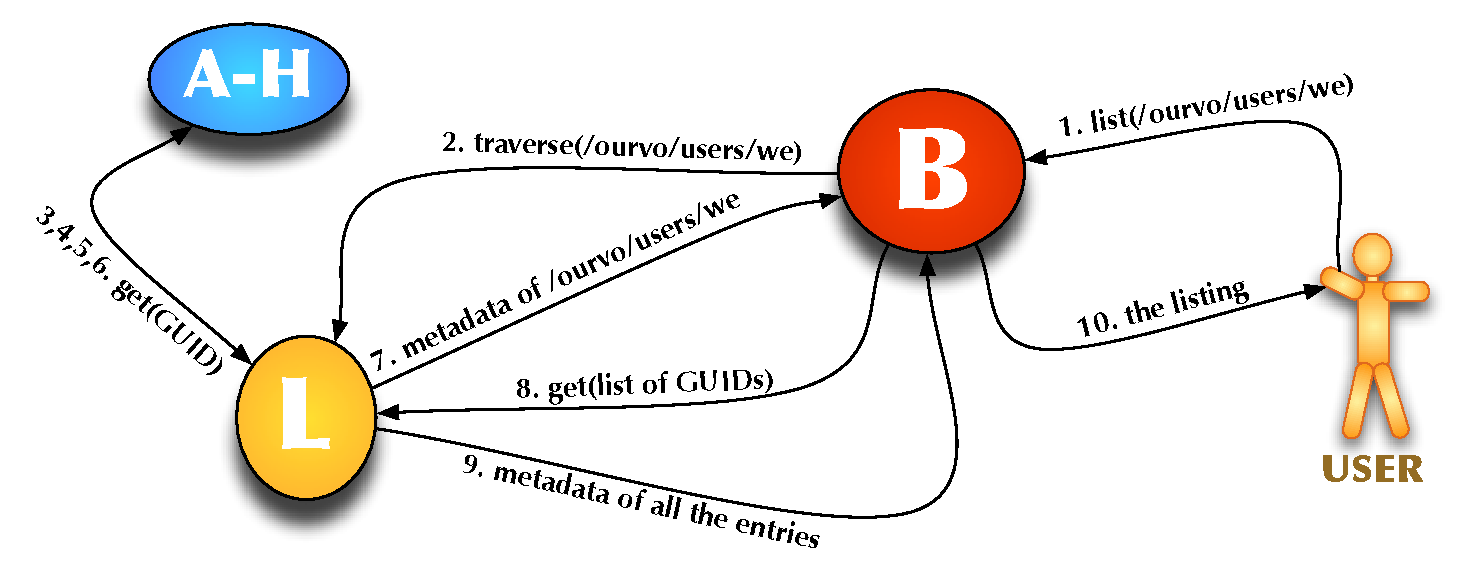
\includegraphics{arc-storage-listing.pdf}}}
\caption{\label{fig:listing}Listing the contents of a collection} }
\end{figure}

A user wants to list the contents of a collection, which has a Logical Name of \verb!/ourvo/users/user!. In order to do this, the client tool has to contact a Bartender, and send a request to it containing the Logical Name the user wants to list, and the response from the Bartender will contain the list of entries. The steps are represented in Figure~\ref{fig:listing}.

\begin{enumerate}
    \item The client tool needs to know the URL of a Bartender. This can be preconfigured on the client side or, in future releases it may be acquired from an information system. When the client tool has the URL, it sends a `list' request which contains the Logical Name \verb!/ourvo/users/user!.
    \item The Bartender tries to get the metadata of the given LN by sending a `traverseLN' request to a Librarian.
    \item The Librarian service starts the traversing by asking an A-Hash service about the first part of the LN, which is the \verb!/! root collection. The A-Hash service only knows about GUID's and not about LN's, but the GUID of the root collection is well-known, so the A-Hash can return the metadata of the list of files and sub-collections in the root collection.
    \item Hopefully, the \verb!ourvo! collection can be found in the root collection, which means that the Librarian knows its GUID, and can ask for its metadata from the A-Hash.
    \item After the A-Hash returns the metadata of the \verb!/ourvo! collection, the Librarian finds the GUID of \verb!users! in it, then gets its metadata.
    \item The A-Hash returns the metadata of \verb!/ourvo/users! which contains the GUID of \verb!user!, so the Librarian can ask for its metadata.
    \item At last the A-Hash returns the metadata of \verb!/ourvo/users/user! to the Librarian, and the Librarian returns it to the Bartender. This metadata contains the list of entries within this collection, and it also contains the access policies for this collection.
    \item The Bartender first checks, based on the user's DN (or his VO membership) and the access policies of this collection, if the user has permission to get the contents of this collection or not. If the user is approved, then because the `list' request should return additional metadata about each entry in the collection, the Bartender sends a `get' message to a Librarian which requests the metadata of all the entries in this collection.
    \item The Librarian gets the metadata from the A-Hash and returns it to the Bartender.
    \item Now the Bartender has all the needed information and returns the proper response to the client tool which formats and prints the results nicely for the user.
\end{enumerate}

% section listing_the_contents_of_a_collection (end)

\section{Downloading a file} % (fold)
\label{sec:downloading_a_file}
\begin{figure}[ht]
\centering{{\scalebox{0.7}{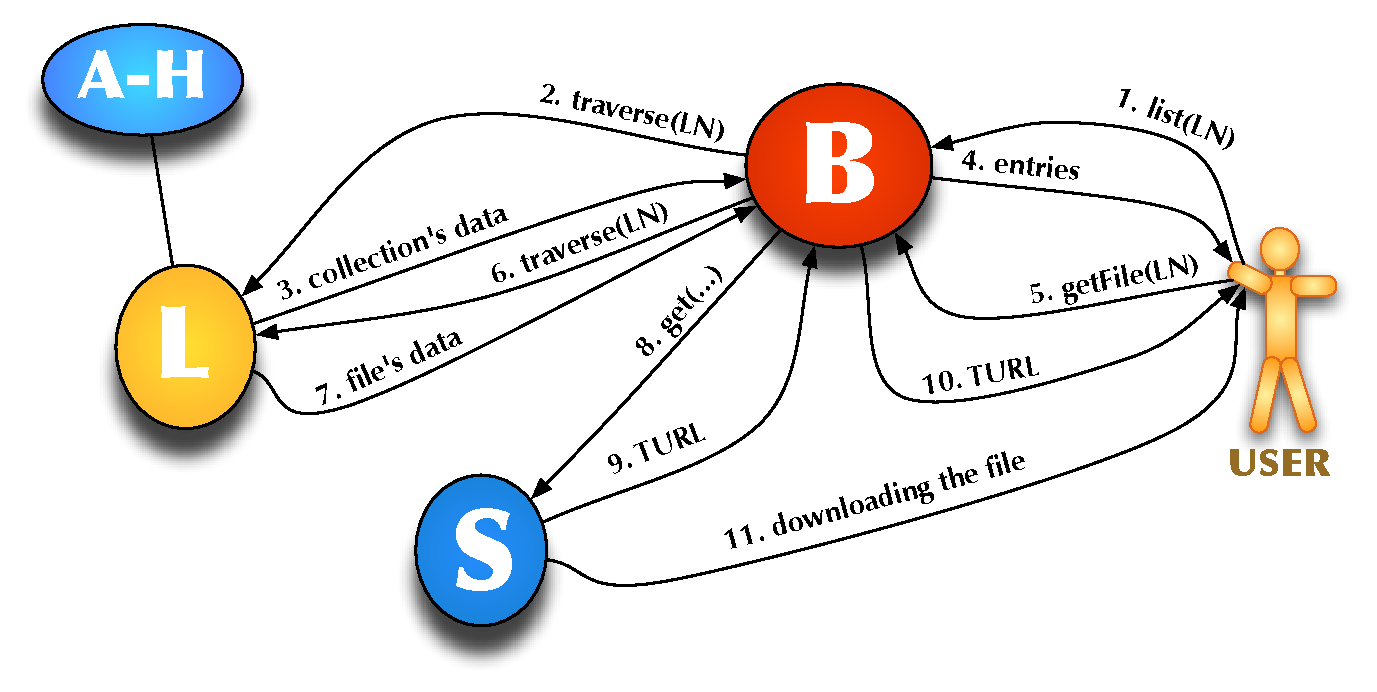
\includegraphics{arc-storage-downloading.pdf}}}
\caption{\label{fig:downloading}Downloading a file} }
\end{figure}

In this use case a user wants to download a file which has a Logical Name of \verb#/ourvo/users/user/thefilehewants# (see Figure~\ref{fig:downloading}).

\begin{enumerate}
    \item The client tool connects to a Bartender and sends a `getFile' request with the LN of the file.
    \item The Bartender contacts a Librarian to traverse the Logical Name and to get the metadata of our file.
    \item The Librarian does the step-by-step traversing of the name space and gets all the metadata from the A-Hash and returns the metadata of our file to the Bartender. This metadata contains the location of the file's replicas and the access policies of this file.
    \item The Bartender checks, based on the access policies and the user's identity, if he is allowed to get the file, and if allowed, it chooses a replica location (currently randomly). A location consists of the URL of a Shepherd service, and the ID of the replica within that Shepherd (which is called a `referenceID'). The Bartender sends a `get' request to the chosen Shepherd.
    \item The Shepherd prepares the file transfer by asking the storage element service to create a new one-time TURL for this replica. The Shepherd returns the TURL to the Bartender.
    \item The Bartender returns the TURL to the client tool.
    \item The client tool use this TURL to get the file directly from the storage element service on the storage node.
\end{enumerate}

% section downloading_a_file (end)

\section{Creating a collection} % (fold)
\label{sec:creating_a_collection}
\begin{figure}[ht]
\centering{{\scalebox{0.7}{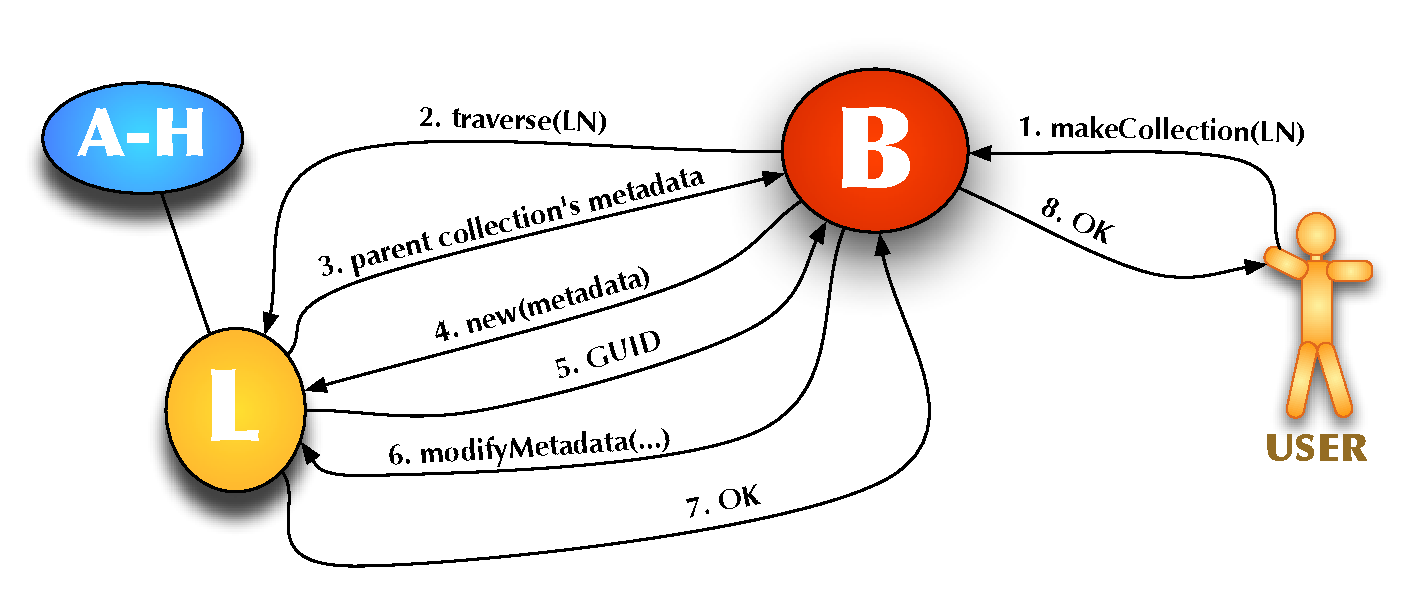
\includegraphics{arc-storage-makecollection.pdf}}}
\caption{\label{fig:makecollection}Creating a collection} }
\end{figure}

Here, the user wants to create a new (empty) collection as sub-collection of \verb#/ourvo/common#, and he wants to call it \verb!docs! (see Figure~\ref{fig:makecollection})

\begin{enumerate}
    \item The client tool contacts a Bartender and send a `makeCollection' request with the LN \verb!/ourvo/common/docs!.
    \item The Bartender asks a Librarian to traverse this LN.
    \item The Librarian tries to traverse the Logical Name and it stops at the last possible point and returns the metadata of the last element. Because the user wants to put his collection in a new path but into an existing collection, we expect that only the \verb#/ourvo/common# part of the LN can be traversed. If the Librarian can traverse the whole LN it means that there is already an existing file or collection by that name. If LN does not exist but the the parent collection does, then the parent collection's metadata is returned to the Bartender. 
    \item The Bartender checks the access policies to decide if the user has permissions to put something into this collection. Then it asks the Librarian to create a new collection.
    \item The Librarian creates the collection, and returns its GUID. At this point this new collection has no real Logical Name, it only has a GUID, but it is not yet put into its parent collection.
    \item The Bartender now asks the Librarian to add this new entry into the parent collection, which means that the new GUID and the name \verb!docs! are added as a pair.
    \item The Librarian returns with a status message.
    \item Finally the Bartender tells the client tool if everything went OK or not.
\end{enumerate}


% section creating_a_collection (end)

\section{Uploading a file} % (fold)
\label{sec:uploading_a_file}

\begin{figure}[ht]
\centering{{\scalebox{0.7}{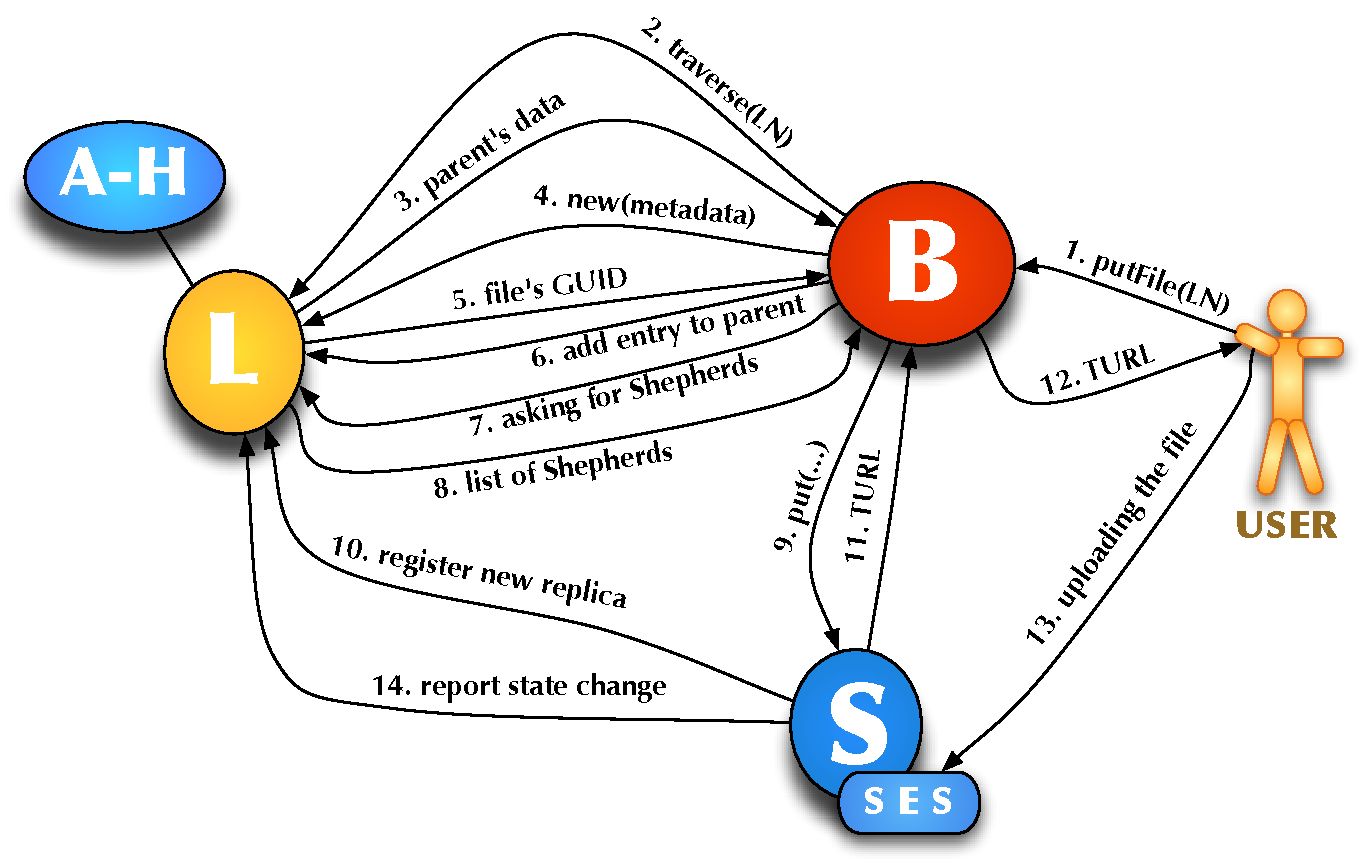
\includegraphics{arc-storage-uploading.pdf}}}
\caption{\label{fig:uploading}Uploading a file} }
\end{figure}

The user has a file on his local disk and wants to upload the file to a collection called \verb#/ourvo/common/docs#. (See Figure~\ref{fig:uploading}.)
\begin{enumerate}
    \item The client tool contact a Bartender to upload the file, providing the file's metadata, including the the Logical Name (LN), which in this case will be \verb#/ourvo/common/docs/proposal.pdf#
    \item The Bartender asks a Librarian to traverse this LN.
    \item The Librarian traverses the Logical Name, and stopping at the \verb#/ourvo/common/docs# part of the LN, which means that the name is available and the parent collection exists. If everything is OK, the metadata of the parent collection is returned to the Bartender. 
    \item The Bartender checks the access policies to decide if the user has permissions to put anything into this collection. Then it asks the Librarian to create a new file entry. 
    \item The Librarian creates the entry and returns its GUID.
    \item Next, the Bartender adds the name \verb#proposal.pdf# and the new GUID to the collection \verb#/ourvo/common/docs# and from now on there will be a valid LN \verb#/ourvo/common/docs/proposal.pdf#. However this LN points to a file which has currently no replica at all. If someone tried to download the file called \verb#/ourvo/common/docs/proposal.pdf# now, they would get an error message.
    \item The Bartender asks the Librarian about Shepherd services (which are sitting on storage nodes).
    \item The Librarian returns a list of Shepherd services.
    \item The Bartender randomly chooses a Shepherd service and sends it a `put' request to initiate the file upload. 
    \item The Shepherd communicates with the storage element service on the same node to create a new transfer URL (TURL). Then it creates a `referenceID' for this file and reports to the Librarian that there is a new replica in the \verb#creating# state. The Librarian gets the message from the Shepherd and adds the new replica to the new file. Now the file has one replica, which is not uploaded yet into the system. If someone tries to download this file now, they still get an error message.
    \item The Shepherd returns the the TURL to the Bartender.
    \item The Bartender returns the TURL to the client tool.
    \item Then client tool can upload the file to this TURL.
    \item The Shepherd detects that the file has been uploaded. In order to do this the storage element service does post processing (e.g. remove a hardlink, do a SOAP call, etc.) after it got the file. The Shepherd checks the checksum of the file, and if it is OK, then it reports to the Librarian, that this replica is now \verb#alive#. The Librarian alters the state of this location, and now the file has one valid replica. 
\end{enumerate}

% section uploading_a_file (end)

\section{Removing a file} % (fold)
\label{sec:removing_a_file}

\begin{figure}[ht]
\centering{{\scalebox{0.7}{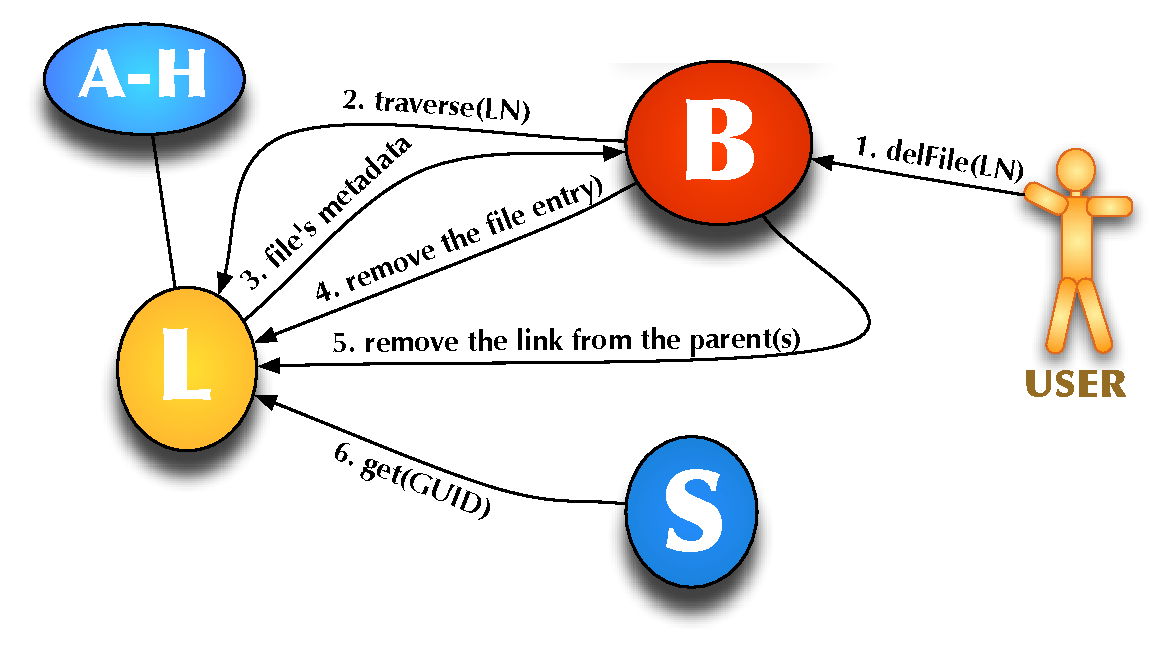
\includegraphics{arc-storage-removing.pdf}}}
\caption{\label{fig:removing}Removing a file} }
\end{figure}
In Chelonia, files are deleted through so called {\it lazy deletion}, meaning that at first only the Logcial Name (LN) is deleted, while the physical replicas are removed at a later stage.
\begin{enumerate}
    \item If the user wants to remove a file, his client tool should connect to a Bartender with the LN of the file he wants to remove.
    \item The Bartender asks the Librarian to traverse the LN.
    \item The Librarian returns the metadata of the file. The metadata contains information about all the hardlinks which points to this file if there are more than one.
    \item Now the Bartender asks the Librarian to remove the file.
    \item After that, the Bartender asks the Librarian to remove the links to this file from all the parent collections.
    \item The next time a Shepherd which has a replica of this file does its periodic check, it asks the Librarian about the file, and notices that the file does not exist anymore, so it removes the replica itself from the storage node.
\end{enumerate}

% section removing_a_file (end)

% chapter use_cases (end)

\chapter{Technical description} % (fold)
\label{cha:technical_description}

\section{Framework and language} % (fold)
\label{sec:framework_and_language}

The Chelonia services are written in Python and execute in the HED\footnote{The ARC container - \url{https://www.knowarc.eu/documents/Knowarc\_D1.2-2\_07.pdf}} hosting environment. The HED itself is written in C++, but there are language bindings which allow services to be written in other languages, e.g.~in Python or Java. The source code of the storage services is in the NorduGrid Subversion repository\footnote{\url{http://svn.nordugrid.org/trac/nordugrid/browser/arc1/trunk/src/services/storage}}.

Because the next-generation information system of ARC is currently under development, it cannot be used to discover services. Hence, currently the URL's of almost all the services are hard-coded in the configuration files of the service. There is one exception: the Shepherd services are reporting their URL's to the Librarians, so a Bartender can always get the most current list of accessible Shepherd services.

The HED has a security framework which the Bartenders use the make access policy decisions. The details of this is described in Section \ref{sec:security_implementation}.

% section framework_and_language (end)

\section{Data model} % (fold)
\label{sec:data_model}

The storage system stores different kinds of metadata about files, collections, mount points, Shepherd services, etc. Each of these has a unique ID; a GUID.

The A-Hash services provide a functionality to store `objects', where each object has a unique ID, and contains property-value pairs organized in sections. The properties, the values and the section names are simple character strings. The A-Hash services provide a simple interface to interact with these objects, e.g.~to do conditional and atomic changes.

The Librarian services use the A-Hash services to store the metadata, using the GUID's as unique ID's. For this, we have to represent the metadata as property-value pairs organized in section. The files, the collections and the mount points have some common attributes: the GUID, the type and the owner which are in the \emph{entry} section; the creation and modification timestamps in the \emph{timestamps} section, a list of access control rules in the \emph{policy} section; the list of parent collections where this entry has a `hardlink' in the \emph{parents} section; and optional, arbitrary property-value pairs in the \emph{metadata} section.

\begin{description}
    \item [entry] section 
    \begin{itemize}
        \item \emph{type}: the type of the entry: `collection', `file' or `mountpoint'
        \item \emph{GUID}: the unique ID of the entry
        \item \emph{owner}: the DN of the user who owns this entry
    \end{itemize}
    \item [timestamps] section 
    \begin{itemize}
        \item \emph{created}: timestamp of creation 
        \item \emph{modified}: timestamp of last modification (the support for this is not implemented yet)
    \end{itemize}
    \item [policy] section 
    \begin{itemize}
        \item \emph{(identity, action list) pairs}: a list of allowed and not allowed actions for different identities (users, VO's, etc., see Section \ref{sub:high_level_authorization} for details). 
    \end{itemize}
    \item [parents] section
    \begin{itemize}
        \item list of GUID's of collection where this entry is located, and the name of this entry within the given collections
    \end{itemize}
    \item [metadata] section 
    \begin{itemize}
        \item optional arbitrary property-value pairs
    \end{itemize}
\end{description}

\subsection{Files} % (fold)
\label{sub:files}

A file in Chelonia has a logical entry in the namespace, and one or more physical replicas on the storage nodes. We store the locations of the replicas in the \emph{locations} section. A location contains the URL of the Shepherd service, the local ID of the file within the storage node and the state of the replica. This state is `\textbf{alive}' if the replica passed the checksum test, and the Shepherd reports that the storage node is healthy, `\textbf{invalid}' if the replica has wrong checksum, or the Shepherd claims it has no such file, `\textbf{offline}' if the Shepherd is not reachable, but may have a valid replica, `\textbf{creating}' if the replica is in the state of uploading, `\textbf{thirdwheel}' if the replica is marked for deletion because of too many replicas, or `\textbf{stalled}' if the the replica was in the state if uploading for a long time but hasn't arrived. The \emph{states} section contains the size of the file, the number of required replicas, and a checksum of the file, which is created by some kind of checksumming algorithm (currently only md5 is supported).

\begin{description}
    \item [locations] section 
    \begin{itemize}
        \item \emph{(location, state) pairs}: where a location is a (\emph{URL}, \emph{referenceID}) pair serialized as a string, where \emph{URL} is the address of the Shepherd service storing this replica, \emph{referenceID} is the ID of the file within that Shepherd service.
    \end{itemize}
    \item [states] section 
    \begin{itemize}
        \item \emph{size}: the file size in bytes
        \item \emph{checksum}: checksum of the file
        \item \emph{checksumType}: the name of the checksum method
        \item \emph{neededReplicas}: how many valid replicas should this file have 
    \end{itemize}
\end{description}


% subsection files (end)


% The Librarian uses the A-Hash to store all the data about files and collections. The A-Hash is capable of storing property-value pairs organized in sections, which actually means that it stores (\emph{section}, \emph{property}, \emph{value}) tuples where each member is simply a string, e.g.~(`entry', `type', `collection') or (`ACL', `johnsmith', `owner') or (`timestamps', `created', `1196265901') or (`locations', `64CDF45F-DDFA-4C1D-8D08-BCF7810CB2AB:9A293F27DC86', `sentenced'). There could be only one \emph{value} for a (\emph{section}, \emph{property}) pair.


\subsection{Collections} % (fold)
\label{sub:collections}

A \emph{collection} is a list of files and other collections, which are in parent-children relationships forming a tree-hierarchy. Each entry has a unique name within a collection and a GUID which points to a corresponding file or collection, so a collection is basically a list of name-GUID pairs, which list is stored in the \emph{entries} section (see below). The collections can be in a closed state, which means that its contents should not be changed. If you close a collection then it cannot be opened again. However it cannot be guaranteed that the contents of a closed collection remains the same (e.g. if we include in our collection a file which we don't own, then the owner of the file can still remove it), but if a closed collection is changed, its state will be broken, and this state can never be changed again, which means you will always know if a closed collection is not intact anymore. This state is stored in the \emph{states} section, and its possible values are `\textbf{no}' if the collection is not closed, `\textbf{yes}' if the collection is closed and `\textbf{broken}' if the collection was closed, but something happened, and its contents have been changed.

\begin{description}
    \item [entries] section 
    \begin{itemize}
        \item \emph{(name, GUID) pairs}: a collection is basically a list of name-GUID pairs. 
    \end{itemize}
    \item [states] section 
    \begin{itemize}
        \item \emph{closed}: this indicates if the collection is closed or broken. 
    \end{itemize}
\end{description}

% subsection collections (end)

\subsection{Mount Points} % (fold)
\label{sub:mount_points}

The mount point entry is a reference to an external third-party storage. Its metadata is basically just the URL of the external storage end point.

\begin{description}
    \item [mountpoint] section 
    \begin{itemize}
        \item \emph{externalURL}: the URL of the external storage end point.
    \end{itemize}
\end{description}


% subsection mount_points (end)

\subsection{Shepherds} % (fold)
\label{sub:shepherds}

The Librarian stores information about the registered Shepherd services. Each Shepherd reports its URL and the list of its files to a Librarian, and for each Shepherd a GUID is created. There is a special entry (with GUID `1' by default) which stores a list of the registered Shepherd services, with their GUID and the timestamp of the last heartbeat message from them.

\begin{description}
	\item [nextHeartBeat] section
	\begin{itemize}
		\item \emph{(URL, timestamp) pairs}: contains when was the last heartbeat of this service
	\end{itemize}
	\item [serviceGUID] section
    \begin{itemize}
        \item \emph{(URL, GUID) pairs}: connects the URL of the Shepherd to the GUID where the information is stored about the Shepherd's stored files
    \end{itemize}
\end{description}

And for each Shepherd there is a separate entry with the list of all files stored on the given storage nodes:

\begin{description}
	\item [entry] section
    \begin{itemize}
        \item \emph{type}: `shepherd'
    \end{itemize}
	\item [files] section
	\begin{itemize}
	    \item \emph{(referenceID, GUID) pairs}: for each replica stored on the Shepherd
	\end{itemize}
\end{description}

% subsection shepherds (end)


% section data_model (end)

\section{Security implementation} % (fold)
\label{sec:security_implementation}

The ARC HED hosting environment has a security framework, and it has its own policy language for describing access policies and requests. The storage system currently use a different internal format to store the access policies, but when the time comes to make decisions, it converts the stored policies and the incoming requests to the ARC native policy format, then asks the security framework to decide.

The internal representation of the access policies is based on access rules. A rule contains an identity and a list of actions. Currently the identity can be one of the following:
\begin{itemize}
    \item a Distinguish Name (DN) of a user, e.g. `\verb!/DC=eu/DC=KnowARC/O=NIIFI/CN=james!'
    \item a name of a Virtual Organization (VO) prefixed with `\verb!VOMS:!', e.g. `\verb!VOMS:knowarc.eu!'
    \item `\verb!ALL!' to specify that this rule will be applied to everyone
    \item `\verb!ANONYMOUS!' for a rule which will be applied to unauthenticated users (e.g. when non-secure HTTP is used and there is no DN)
\end{itemize}

Then for each rule there is list of actions, each action is either allowed or denied. In the internal representation of an access rule the list of actions is one single string, where the name of actions are separated with a space, and each name is prefixed with a `\verb!+!' or `\verb!-!' sign indicating if the action is allowed or denied for the given identity. The list of actions can be found in section~\ref{sub:high_level_authorization}.

When there is an incoming connection to a Bartender, the security framework of the HED extracts the identity information of the connecting client (DN of client, DN of the issuer CA, extended attributes, etc.), and all this information is accessible by the Bartender. When the given method of the Bartender gets to the point where the access rules are present, and it is clear that what kind of action the user wants to do, then both the request and the policy are converted to the native ARC policy language, and then the policy evaluator of the security framework is called to make the decision. The native ARC policy language defines attribute types for attributes within requests and policies. The XML representation of an ARC policy or request contains several `Attribute' elements, each have a type and a value. The storage actions are also put into Attribute elements with the type `\verb!http://www.nordugrid.org/schemas/policy-arc/types/storage/action!'.

For inter-service authorization the services can be configured to only accept connections from trusted services. A service is trusted if we know its DN. For each service we can write trusted DN's in the configuration, or we can periodically get the list from an A-Hash. This can be configured with a `\emph{TrustManager}' section in the service configuration, which contains these entries:

\begin{description}
    \item[DN] is a trusted DN
    \item[CA] is a DN of a trusted CA: all certificates issued by this CA are trusted
    \item[DNsFromAHash] is a list of A-Hash URL's (in \textbf{AHashURL}) from where a list of trusted DN's are periodically obtained (there can be multiple A-Hash URL's listed here in case of one is offline). The following attributes are obtained: \textbf{CheckingInterval} specifies how frequently the list from the A-Hash should be updated (default: 600 seconds); \textbf{ID} specifies the GUID where the list is stored (default: `3').
\end{description}

The TrustManager section itself have the following optional attributes: \textbf{FromFile} can specify a filename if we want to get the whole TrustManager configuration from a separate file; and \textbf{Force} indicates (with `yes' or `no', default: `yes') that we want to ensure that our service does not even get the request if the client of the incoming connection is not trusted. 

Example TrustManager configuration:

\begin{verbatim}
    <TrustManager Force="yes">
        <DN>/DC=eu/DC=KnowARC/O=NIIFI/CN=host/epsilon</DN>
        <DN>/DC=eu/DC=KnowARC/O=NIIFI/CN=host/phi</DN>
        <CA>/DC=eu/DC=KnowARC/CN=storage-1233659377.11</CA>
        <DNsFromAHash CheckingInterval="10">
            <AHashURL>https://localhost:60000/AHash</AHashURL>
        </DNsFromAHash>
    </TrustManager>
\end{verbatim}

All the services must have their own X.509 certificates, which they use when connecting to other services. Currently, it is needed to set the paths of the certificate and private key files (and the trusted CAs as well) in the configuration of each service, like this:

\begin{verbatim}
    <ClientSSLConfig>
        <KeyPath>certs/hostkey-epsilon.pem</KeyPath>
        <CertificatePath>certs/hostcert-epsilon.pem</CertificatePath>
        <CACertificatesDir>certs/CA</CACertificatesDir>
    </ClientSSLConfig>
\end{verbatim}

This can be put in a separate file, and then use the \textbf{FromFile} attribute of the ClientSSLConfig section to specify where the file is.

% section security_implementation (end)

\newpage

\section{A-Hash} % (fold)
\label{sec:a_hash}

\subsection{Functionality} % (fold)

The A-Hash is a database for storing string tuples, and it provides conditional and atomic modification of them. The A-Hash can be used as a centralized service, or it can be deployed in a distributed way, using multiple nodes, where all the data is replicated on all the nodes.

The A-Hash stores \emph{objects}, where each object has an arbitrary string \emph{ID}, and contains any number of \emph{property}-\emph{value} pairs grouped in \emph{section}s, where \emph{property}, \emph{value} and \emph{section} are arbitrary strings. It can only be one \emph{value} for a \emph{property} in a \emph{section}.

Given an ID, the \emph{get} method returns property-value pairs of the corresponding object. By specifying a section or property, the \emph{get} method returns the corresponding values. Using the \emph{change} method, property-value pairs can be added and removed from an object, all occurrences of a property can be deleted and new objects can be created. By specifying conditions, the change is only applied if the given conditions are met.

% subsection functionality (end)

\subsection{Interface} % (fold)

\begin{description}
    \item [get(IDs, neededMetadataList)] returns all or some of the property-value pairs of the requested objects.
    
    The \emph{IDs} is a list of string \emph{ID}'s, \emph{neededMetadataList} is a list of (\emph{section}, \emph{property}) pairs. If the \emph{neededMetadataList} is empty, then for each \emph{ID} it returns all the \emph{values} for all the \emph{properties} in all the \emph{section} in that given object. If there are sections and properties specified in \emph{neededMetadataList}, then only those values are returned.

    The response contains a list of \emph{object}s, where an \emph{object} is an (\emph{ID}, \emph{metadataList}) pair, where \emph{metadataList} is a list of (\emph{section}, \emph{property}, \emph{value}) tuples.

    \item [change(changeRequestList)] modifies, removes or creates objects if certain conditions are met, and returns information about the success of the modification requests.
    
    The \emph{changeRequestList} is a list of \emph{changeRequest}s, where a \emph{changeRequest} is a tuple of (\emph{changeID}, \emph{ID}, \emph{changeType}, \emph{section}, \emph{property}, \emph{value}, \emph{conditionList}):
\begin{itemize}
\item \emph{changeID} is an arbitrary ID which is used in the response to refer to this part of the request
\item \emph{ID} points to the object we want to change
\item \emph{changeType} can be `\textbf{set}' to set the property within the section to value, `\textbf{unset}' to remove the property from the section regardless of the value, `\textbf{delete}' to remove the whole object
\item \emph{conditionList} is a list of \emph{condition}s, where a \emph{condition} is a tuple of (\emph{conditionID}, \emph{conditionType}, \emph{section}, \emph{property}, \emph{value}), where \emph{conditionType} can be `\textbf{is}' which will be true if the property in the section is set to the value, `\textbf{isnot}' which will be true if the property in the section is not set to the value, `\textbf{isset}' which will be true if the property of the section is set regardless of the value or `\textbf{unset}' which will be true if the property of the section is not set at all.
\end{itemize}
    If all conditions are met, the A-Hash tries to apply changes to the objects, and creates a new object if a previously non-existent ID is given.
    
    The response contains the \emph{changeResponseList} which is a list of (\emph{changeID}, \emph{success}, \emph{failedConditionID}) tuples. The \emph{success} of the change is either \textbf{set}, \textbf{unset}, \textbf{deleted}, \textbf{failed}, \textbf{condition not met} (in which case the ID of the failed condition is put into \emph{failedConditionID}), \textbf{invalid change type} or \textbf{unknown}.
    
    
\end{description}
    
% subsection interface (end)

\subsection{Implementation} % (fold)

The A-Hash service has a modular architecture which means that it can be deployed in a centralized or a distributed way by simply specifying different modules in the service's configuration. There are different low-level modules for storing the metadata on disk, e.g. serialized into the `pickle' format. In addition there is a module which stores the metadata replicated on multiple nodes.

The replicated A-Hash module is built on Oracle Berkeley DB High Availability, an open source database library with a replication API. The replication is based on a single master, multiple clients framework where all clients can read from the database, while only the master is allowed to write to the database. This ensures that all database transactions are ACID (atomic, consistent, isolated and durable). The replicated A-Hash module consists of three modules, \verb!ReplicatedAHash!, \verb!ReplicationStore! and \verb!ReplicationManager!.

\begin{description}
    \item[ReplicatedAHash] 
	is a subclass of the \verb!CentralizedAHash! business logic class and implements the extra logic needed for communication between A-Hash instances. The \verb!ReplicatedAHash! adds the method \verb!sendMessage! to the A-Hash interface and has a method \verb!processMessage! for processing messages from \verb!sendMessage!. These two methods are needed for the communication framework of the \verb!ReplicationManager!. The actual replication is managed by the \verb!ReplicationStore! and \verb!ReplicationManager!, meaning that the \verb!ReplicatedAHash!, with the exception of the above-mentioned methods, is actually just a centralized A-Hash with a specific storage module.
    \item[ReplicationStore] 
	is a specialized replicated database. It is a subclass of \verb!TransDBStore!\footnote{A module for storing data on disk transactionally using the Berkeley DB library.} with some additional features for handling replication. The \verb!ReplicationStore! periodically updates an A-Hash object which contains information about the current master A-Hash and available clients. In addition it contains a \verb!ReplicationManager! object which governs the replication framework.
    \item[ReplicationManager] 
	handles all aspects of the Berkeley DB API and takes care of replicas, elections of the master replica and replication messages.
	\begin{itemize}
	\item The replicated A-Hash consists of a set of replicas; one master and multiple clients. This means that the entire database is fully replicated on all replicas. When the master receives a write message, it will broadcast this message to all the clients. To make sure that the database is consistent and that it will always be possible to elect a master, the master requires an acknowledgement message from a quorum of clients before continuing.
	\item In the replicated A-Hash there is one master and multiple clients. When the A-Hash starts up or if a master goes offline, a new master must be elected. This is solved by the clients holding an election, according to the Paxos algorithm\footnote{http://research.microsoft.com/users/lamport/pubs/pubs.html\#lamport-paxos}. Simply told, all clients send a vote to all other clients, and the eligible client that gets the most votes wins the election. An eligible client is a client which has received the latest updates. See the Berkeley DB documentation for more details. There are cases where some servers are more suitable to be master than others (better hardware, faster Ethernet, etc.). In such cases the election can be influenced by setting a higher priority on the best servers. While an election is being held, it is not possible to write to or read from the A-Hash, as consistency cannot be guaranteed without a master.
	\item As the replicas in the replicated A-Hash are services running within HED, the replication messages need to be sent through the communication framework of HED. To be able to use this framework, the Berkeley DB needs a callback function for sending messages and the \verb!ReplicationManager! needs to call Berkeley DB to process incoming messages. The \verb!ReplicationMessage! takes a send function as one of the initialization arguments, and calls this function in the callback method. By providing the \verb!ReplicatedAHash.sendMessage! to the \verb!ReplicationManager! messages will be sent through the HED communication services just as in regular inter service communication. When \verb!ReplicatedAHash! receives a replication message from \verb!sendMessage! it will call \verb!ReplicationManager.processMessage! which in turn will call the Berkeley DB processMessage. This communication framework is both used by Berkeley DB and directly by the \verb!ReplicationManager!, e.g., for bootstrapping the A-Hash replicas and to communicate newly discovered clients.
\end{itemize}
\end{description}

% subsection implementation (end)

\subsection{Configuration} % (fold)
\label{sub:a_hash_configuration}


The A-Hash has the following configuration variables:

\begin{description}
    \item[AHashClass] tells the A-Hash service the name of the business-logic A-Hash class. Currently there are two implementation, the \verb!CentralAHash! is a centralized version, and the \verb!ReplicatedAHash! is a replicated version.
    \item[StoreClass] specifies the name of the store class, used to store the data on disk. Currently there are several store classes each has the same interface but uses different mechanisms (\verb!PickelStore!, \verb!CachedPickleStore!, \verb!StringStore!, \verb!ZODBStore!, \verb!TransDBStore!), however only the \verb!TransDBStore! class is suitable for use in a replicated deployment. All the others are only for a centralized deployement, so this variable is only configurable for the centralized deployement. Based on our tests, currently the \verb!CachedPickleStore! has the best performance.
    \item[StoreCfg] contains parameters for the different store classes, and it almost always contains a \emph{DataDir} parameter which specifies a directory on the (local) filesystem where the A-Hash can save its files. This variable is only configurable for the centralized deployment.
\end{description}

For the replicated A-Hash there are some additional mandatory configuration variables:

\begin{description}
    \item[LocalDir] specifies a directory on the local filesystem where this A-Hash replica should be stored. This directory must be unique for this replica, i.e., no two A-Hash replicas can share the same \verb!LocalDir! since doing so will most likely leave both replicas broken beyond repair.
    \item[MyURL] is the URL to this A-Hash service and is used as an ID for this service in the replication group.
    \item[OtherURL] is the URL of another A-Hash in the replication group. More than one URL can be specified here.
\end{description}

Even though the default settings are useable, there are some optional variables available for the replicated A-Hash:
\begin{description}
    \item[Priority] is related to the master election. If a master dies, there will be an election to decide which client will be the new master. Higher priority means a higher chance to be elected. A priority of 0 means that this replica can never be elected. The defaults is 10.
    \item[CheckPeriod] specifies in seconds how frequently the A-Hash should update the replica list. The default is 10 seconds.
    \item[CacheSize] configures the amount of the storage to be cached in memory. The default is 10MB
\end{description}


Example of a centralized A-Hash configuration:

\begin{verbatim}
    <Service name="pythonservice" id="ahash">
        <ClassName>storage.ahash.ahash.AHashService</ClassName>
        <AHashClass>storage.ahash.ahash.CentralAHash</AHashClass>
        <StoreClass>storage.store.cachedpicklestore.CachedPickleStore</StoreClass>
        <StoreCfg>
            <DataDir>ahash_data</DataDir>
        </StoreCfg>
    </Service>
\end{verbatim}

Example of a replicated A-Hash configuration:
\begin{verbatim}
    <Service name="pythonservice" id="ahash1">
        <ClassName>storage.ahash.ahash.AHashService</ClassName>
        <AHashClass>storage.ahash.replicatedahash.ReplicatedAHash</AHashClass>
        <LocalDir>ahash_data1</LocalDir>
        <MyURL>http://localhost:60000/AHash1</MyURL>
        <OtherURL>http://localhost:60001/AHash2</OtherURL>
        <Priority>50</Priority>
        <ClientSSLConfig FromFile='clientsslconfig.xml'/>
    </Service>
\end{verbatim}

% subsection configuration (end)

% section a_hash (end)
\newpage

\section{Librarian} % (fold)
\label{sec:librarian}

\subsection{Functionality} % (fold)
% 

The Librarian knows about the type of possible entries in the namespace of Chelonia: files, collections and mount points. It knows that these are organized in a tree-hierarchy with entries grouped into collections, and it knows about Logical Names, and how to traverse a Logical Name to find the metadata of the file or collection (or mount point) which it refers to. However, the Librarian does not maintain the namespace of Chelonia. It does not put new files into collections, nor remove the link from its parent collection when a file is removed - this is the job of the Bartender. The only Librarian method which deals with Logical Names is the \emph{traverseLN} method, which traverses the Logical Name as far as possible, and returns the GUID and metadata of the last found entry in the path of the Logical Name. All the other methods work with GUID's, and do not care about the hierarchical namespace. In this regard the Librarian can be treated as a higher level application-specifc interface to the metadata store (the A-Hash), because while the A-Hash does not care about what it stores, the Librarian knows exactly that it stores metadata about files, collections, etc. With this interface new files, collections and mount points can be created with the \emph{new} method, the metadata of any entry can be retrieved and modified with the \emph{get} and \emph{modifyMetadata} methods, and entries can be removed with the \emph{remove} method.

Besides being an interface to the metadata store, the Librarian has another important functionality: it provides a way for Shepherds to register themselves and to periodically send reports about the state of their stored files. A Shepherd sends a \emph{report} message to a Librarian if e.g. a new file arrived, or an old file gets corrupted, thus the Librarian can keep the states of the replicas up-to-date. The Librarian monitors the registered Shepherds, and if one of them stops sending reports, the Librarian will assume, that it is offline, and modify the states of all the replicas which are on the Shepherd's storage node. In order to do this, the Librarian stores for each Shepherd a list of files on the given storage nodes, this make it possible to know which files have replicas on a given storage nodes without checking all the files in the system. This list of files gets updated every time a Shepherd sends a report.

The end-user of Chelonia never communicates directly with a Librarian, the Bartenders will contact the Librarians in order to fulfil the user's requests.

% subsection functionality (end)

\subsection{Interface} % (fold)

\begin{description}

    \item [get(getRequestList, neededMetadataList)] returns all or some of the metadata of the requested GUID's.
    
    The \emph{getRequestList} is a list of string \emph{GUID}'s, \emph{neededMetadataList} is a list of (\emph{section}, \emph{property}) pairs. If \emph{neededMetadataList} is empty, then for each \emph{GUID} all the metadata values for all the properties in all the sections are returned. If there are sections and properties specified in \emph{neededMetadataList}, then only those values are returned.

    The response contains a list of \emph{GUID, metadataList} pairs, where \emph{metadataList} is a list of (\emph{section}, \emph{property}, \emph{value}) tuples.

    \item[new(newRequestList)] creates a new entry in the Librarian with the given metadata, and returns the GUID's of the new entries.
    
    The \emph{newRequestList} is a list of (\emph{requestID}, \emph{metadataList}) where \emph{requestID} is an arbitrary ID used to identify this request in the list of responses; \emph{metadataList} is a list of (\emph{section}, \emph{property}, \emph{value}) tuples.
    This method generates a \emph{GUID} for each request, and inserts the new entry (with the given metadata) into the A-Hash, then returns the GUID's of the newly created entries. In the metadata of the new entry the `type' property in the `entry' section defines whether it is a file, a collection or a mount point. The `GUID' property can contain a GUID if we want to specify the GUID of the new entry, and don't want the Librarian to generate a random one.
    
    The response contains a list of (\emph{requestID}, \emph{GUID}, \emph{success}) tuples.
    
    \item[modifyMetadata(modifyMetadataRequestList)] modifies the metadata of the given entries.
    
    \emph{modifyMetadataRequestList} is a list of (\emph{changeID}, \emph{GUID}, \emph{changeType}, \emph{section}, \emph{property}, \emph{value}) tuples where \emph{changeType} can be `\textbf{set}' to set the property in the section to value, `\textbf{unset}' to remove the property-value pair from the section, `\textbf{add}' to set the property in the section to \emph{value} only if it does not exist already or `\textbf{setifvalue}=value' to only set the property in the section to value if it currently equals to the `value' in the \emph{changeType}.

    The response is a list of (\emph{changeID}, \emph{success}) pairs where \emph{success} can be `\textbf{set}', `\textbf{unset}', `\textbf{condition failed}', `\textbf{failed}: reason'.
    
    \item [remove(removeRequestList)] removes the given entries.

    The \emph{removeRequestList} is a list of (\emph{requestID}, \emph{GUID}) pairs.
    
    The response is a list of (\emph{requestID}, \emph{success}) pairs where \emph{success} is either `\textbf{removed}' or `\textbf{failed}: reason'.
        
    \item [traverseLN(traverseRequestList)] traverses the given Logical Names and returns extensive information about them.
    
    The \emph{traverseRequestList} is a list of (\emph{requestID}, \emph{LN}) pairs with the Logical Names to be traversed
    
    The response is a list of (\emph{requestID}, \emph{traversedList}, \emph{wasComplete}, \emph{traversedLN}, \emph{GUID}, \emph{metadataList}, \emph{restLN}) tuples where:
    \begin{description}
        \item[traversedList] is a list of (\emph{LNpart}, \emph{GUID}) pairs, where \emph{LNpart} is a part of the \emph{LN}, \emph{GUID} is the GUID of the Librarian-entry referenced by that part of the \emph{LN}, the first element of this list is the shortest prefix of the \emph{LN}, the last element is the \emph{traversedLN} without its last part
        \item[wasComplete] indicates whether the full \emph{LN} was traversed
        \item[traversedLN] is the part of the \emph{LN} which was traversed, if \emph{wasComplete} is true, this should be the full \emph{LN}
        \item[GUID] is the \emph{GUID} of the \emph{traversedLN}
        \item[metadataList] is all the metadata of the of traversedLN in the form of (\emph{section}, \emph{property}, \emph{value}) tuples
        \item[restLN] is the remainders of the \emph{LN} which was not traversed for some reason, if \emph{wasComplete} is true, this should be an empty string
    \end{description}
    
    \item [report(serviceID, filelist)] is a report message from a Shepherd to a Librarian which contains the ID of the Shepherd, and a list of changed files on the Shepherd's storage node.
        
    The \emph{filelist} is a list of (\emph{GUID}, \emph{referenceID}, \emph{state}) tuples containing the state of changed or new files, where referenceID is the Sheperd-local ID of the given replica and GUID refers to the logical file of this replica. The \emph{state} is one of `\textbf{invalid}' (if the periodic self-check of the Shepherd found a non-matching checksum or missing file), `\textbf{creating}' (if this is a new file not uploaded yet), `\textbf{thirdwheel}' (if the replica is marked for deletion because of too many replicas), `\textbf{alive}' (if the file is uploaded and the checksum is OK), or `\textbf{stalled}' (if the file was in `creating' state for a long time but hasn't arrived).
    
    The response is \emph{nextReportTime}, a number of seconds, which is the timeframe within which the Librarian expects to receive the next heartbeat from the Shepherd.

\end{description}

% subsection interface (end)

\subsection{Implementation} % (fold)

The Librarian service uses the A-Hash to store all the metadata, and it uses the GUID's as ID's in the database. It has the URL of one or more A-Hash services in its configuration, and it can acquire more A-Hash URL's from these first A-Hashes in case of a replicated A-Hash deployment.

The replicated A-Hash deployment is based on a single master, multiple clients scenario (see Section~\ref{sec:a_hash} for details). This means that the Librarian can read from any A-Hash, while it can only write to the master A-Hash. A list of A-Hashes, master and clients, is stored in an A-Hash object. The Librarian periodically retrieves this list to maintain its own list of A-Hash services. If the Librarian tries to write to the replicated A-Hash and the master is down, the Librarian will try to get a new list from one of the clients and retry the write request once before giving up. In case of reading from the replicated A-Hash, the Librarian will randomly loop through the list of clients until the read request is successful or until there are no more clients available.

The Librarian also accepts report messages from Shepherds, and stores the contents of these messages in the A-Hash. There is one A-Hash object which contains the ID and the expected time of the next heartbeat of the registered Shepherds, and there is one A-Hash object for each Shepherd which stores the states and GUID's of the files on the Shepherd's storage node (see Section~\ref{sub:shepherds} for details). The Librarian checks periodically if there is a Shepherd which is late with its heartbeat, and it changes the states of all the replicas if needed.

Because the Librarian services store everything in the A-Hash, the Librarian itself is a stateless service. Multiple Librarians may be deployed. If they are configured to use the same replicated group of A-Hashes (or the same central A-Hash) then the Bartenders can use any Librarian to achieve the same results, and the Shepherds can report to any of them. One Shepherd should only report to one Librarian, but if that Librarian is offline, it should find another. The reports will be registered in the A-Hash as well, so it does not matter which Librarian receives a report.

% subsection implementation (end)

\subsection{Configuration} % (fold)

The Librarian has the following configuration variables:

\begin{description}
    \item[AHashURL] is the URL of an A-Hash which the Librarian should use. Multiple A-Hashes may be specified.
    \item[HeartbeatTimeout] specifies in seconds how frequently the Sheperds should send reports to the Librarian.
    \item[CheckPeriod] specifies in seconds how frequently the Librarian should check for late heartbeats.
\end{description}

An example configuration:

\begin{verbatim}
    <Service name="pythonservice" id="librarian">
        <ClassName>storage.librarian.librarian.LibrarianService</ClassName>
        <AHashURL>https://localhost:60000/AHash</AHashURL>
        <HeartbeatTimeout>30</HeartbeatTimeout>
        <CheckPeriod>20</CheckPeriod>
        <ClientSSLConfig FromFile="clientsslconfig.xml"/>
    </Service>
\end{verbatim}

% subsection configuration (end)

% section librarian (end)
\newpage

\section{Shepherd} % (fold)
\label{sec:shepherds}

\subsection{Functionality} % (fold)

A Shepherd service is capable of managing a storage node. It keeps track of all the files it stores with their GUID's and checksums. It periodically checks each file to detect corruptions, and sends reports to a Librarian indicating that the storage node is up and running, and whether the state of any files have been changed. If a file goes missing or has a bad checksum then the Librarian is notified about the error\footnote{Here the Shepherd refers to the file with its GUID, that's why it needs to store the GUID's of its files.}. It periodically asks the Librarian how many replicas its files have, and if a file has fewer replicas than needed, the Shepherd offers its copy for replication by calling the Bartender.

A Shepherd service is always connected to a storage element service (e.g., a web server). For each supported storage element service there is a backend module which makes the Shepherd capable of communicating with the storage element to initiate file transfers, to detect whether a transfer was successful or not, to generate local ID's and checksums and so forth.

A file in a storage node is identified with a \emph{referenceID} which is unique within that node. The \emph{location} of a file consists of the \emph{serviceID} of the Shepherd and the \emph{referenceID}. If the location is known, the Shepherds \emph{get} method can be called with the \emph{referenceID} and a list of transfer protocols, the Shepherd chooses a protocol from this list, and creates a transfer URL (\emph{TURL}). This TURL is returned together with the \emph{checksum} of the file. A client tool may then download the file from this \emph{TURL}, and verify it with the \emph{checksum}. The client tool does not need to call the \emph{get} method. The client tool simply queries the Bartender, which in turn calls the \emph{get} method and returns the TURL.

Storing a file starts with initiating the transfer with the \emph{put} method of the Shepherd, providing the file \emph{size}, the \emph{checksum} of the file and its \emph{GUID}. The client tool also specifies a list of transfer protocols it is able to use, and the Shepherd chooses a \emph{protocol}, creates a \emph{TURL} for uploading and generates a \emph{referenceID}, so that the client tool can upload the file to the TURL. Again, the client tool just asks the Bartender, and gets the TURL; the client tool does not need to call the \emph{put} method of the Shepherd directly.

These \emph{TURL}'s are one-time URL's which means that after the client tool uploads or downloads the file these \emph{TURL}'s cannot be used again to do the same. If the same file is to be downloaded twice, the transfer has to be initiated twice, yielding in two different \emph{TURL}'s.

The \emph{stat} method provides information about a replica, e.g., checksum, GUID, state, etc. The \emph{delete} method removes the replica.

In normal operation the \emph{put} and \emph{get} calls are made by a Bartender but the actual upload and download is done by the client tool. In the case of replication a Shepherd with a valid replica initiates the replication. This Shepherd asks the Bartender to choose a new Shepherd, the Bartender initiates putting the new replica on a chosen Shepherd and receives the TURL, and the Bartender returns the TURL to the initiator Shepherd, which uploads its replica to the given TURL.

The replicas have a state, which is one of `\textbf{creating}' when the transfer is initiated but the file is not uploaded yet, `\textbf{alive}' if the file is uploaded and has a proper checksum, `\textbf{invalid}' if it does not exists anymore or has a bad checksum, `\textbf{thirdwheel}' if the replica is marked for deletion because the file has too many replicas, or `\textbf{stalled}' if it has been in the `creating' state for a long time but hasn't arrived.

% subsection functionality (end)

\subsection{Interface} % (fold)

\begin{description}
    
    \item[get(getRequestList)] initiates a download and returns the TURL
    
    The \emph{getRequestList} is a list of (\emph{requestID}, \emph{getRequestData}) pairs where \emph{requestID} is an arbitrary ID used in the reply, \emph{getRequestData} is a list of (\emph{property}, \emph{value}) pairs, where mandatory properties are: `\textbf{referenceID}' which refers to the file to get and `\textbf{protocol}' indicates a protocol the client can use. getRequestData may contain multiple protocols.
    
    The response is a list of (\emph{requestID}, \emph{getResponseData}), where \emph{getResponseData} is a list of (\emph{property}, \emph{value}) pairs, where \emph{property} may be one of the following: 
    \begin{itemize}
      \item `\textbf{TURL}' is a transfer URL which can be used by the client to download the file
      \item `\textbf{protocol}' is the protocol of the TURL; `\textbf{checksum}' is the checksum of the replica
      \item `\textbf{checksumType}' is the name of the checksum method
      \item `\textbf{error}' contains an error message if there is one.
    \end{itemize}
    \item[put(putRequestList)] initiates an upload and returns the TURL.
        
    \emph{putRequestList} is a list of (\emph{requestID}, \emph{putRequestData}) pairs where \emph{requestID} is an ID used for the response,     \emph{putRequestData} is a list of (\emph{property}, \emph{value}) pairs where property can be one of `\textbf{GUID}', `\textbf{checksum}', `\textbf{checksumType}', `\textbf{size}' (the size of the file in bytes), `\textbf{protocol}' (a protocol the client can use, can be multiple) and `\textbf{acl}' (which is currently not used).
    
    The response is a list of (\emph{requestID}, \emph{putResponseData}) pairs, where \emph{putResponseData} is a list of (\emph{property}, \emph{value}) pairs where \emph{property} may be one of the following:
    \begin{itemize}
      \item `\textbf{TURL}' is the transfer URL where the client can upload the file
      \item `\textbf{protocol}' is the chosen protocol of the TURL
      \item `\textbf{referenceID}' is the generated ID for this new replica
      \item `\textbf{error}' contains an error message.
    \end{itemize}
    \item[delete(deleteRequestList)] removes a replica.
    
    The \emph{deleteRequestList} is a list of (\emph{requestID}, \emph{referenceID}) pairs containing the ID's of the files to remove.
    
    The response is a list of (\emph{requestID}, \emph{status}) pairs, where \emph{status} can be either `\textbf{deleted}' or `\textbf{nosuchfile}'.
    .
    \item[stat(statRequestList)] returns information about replicas.

    \emph{statRequestList} is a list of (\emph{requestID}, \emph{referenceID}) pairs where \emph{referenceID} points to the file whose metadata are requested. 
    
    The response is a list of (\emph{requestID}, \emph{referenceID}, \emph{state}, \emph{checksumType}, \emph{checksum}, \emph{acl}, \emph{size}, \emph{GUID}, \emph{localID}) tuples.
\end{description}

% subsection interface (end)

\subsection{Implementation} % (fold)
\label{sub:shepherd_implementation}

The Shepherd communicates with storage element services via backend modules. Currently there are two backend modules implemented, one for the \emph{Hopi} service\footnote{Note that the Hopi service needs to be configured in a special `slave' mode to be used as a backend for the Shepherd.} (which is a simple HED-based HTTP server), one for the \emph{Apache} webserver\footnote{\url{http://www.apache.org/}}.

In both cases the Shepherd and the transfer services should have access to the same local filesystem where the Shepherd creates two separate directories: one for storing all the files (e.g.~\verb!./store!) and one for the file transfers (e.g.~\verb!./transfer!). The store directory always contains all the files the Shepherd manages, the transfer directory is empty at the beginning.

If a client asks for a file called \verb!file1!, and this file is in the store directory (\verb!./store/file!), the Shepherd service creates a hardlink into the transfer directory (\verb!./transfer/abc!) and sets this file read-only. If the Hopi service is configured to serve the HTTP path \verb!/prb! and it is serving files from the directory \verb!./transfer! then after the hardlink is created, the transfer URL for this file reads \verb!http://localhost:60000/prb/abc!. Now this URL is passed to the client. Then the client \verb!GET!'s this URL and gets the file. The Hopi service removes (unlinks) this file immediately after the \verb!GET! request arrived, which makes \verb!http://localhost:60000/prb/abc! invalid (so this is a one-time URL). However, because of the hardlink the file is still in the store directory, it is just removed from the transfer directory. Now if some other user wants this file, the Shepherd creates an other hardlink, e.g., \verb!./transfer/qwe! with the URL \verb!http://localhost:60000/prb/qwe!.

If a client wants to upload a new file, the Shepherd creates an empty file in the store directory, e.g.~\verb!./store/file2! and creates a hardlink in the transfer directory, e.g., \verb!./transfer/oiu! and makes it writable. The transfer URL is then \verb!http://localhost:60000/prb/oiu!, and the client can do a \verb!PUT! on this URL. When the client tool \verb!PUT!s the file there, the Hopi service immediately removes the uploaded file from the transfer directory, but because it has a hardlink in the store directory, the file is stored there as \verb!./store/file2!. The backend module for the Hopi service periodically checks whether a new file has two hardlinks  or just. If it has only one hardlink that means that the file is uploaded, so it will notify the Shepherd that the file has arrived. In order to do that, the Shepherd needs to provide a callback method `file\_arrived' to the backend module.

All the backend modules should have the following common interface which the Shepherd can use to communicate with the storage element services:

\begin{description}
    \item[prepareToGet(referenceID, localID, protocol)] returns a one-time \emph{TURL}.
    
    Initialize transfer with \emph{protocol} for the file identified by (\emph{localID}, \emph{referenceID}). The reason for including here the referenceID as well is that this information may be used by the backend module later, e.g., when the transfer has finished and the state of the file needs to be changed.
    
    \item[prepareToPut(referenceID, localID, protocol)] returns a one-time \emph{TURL}.
    
    Initialize transfer with \emph{protocol} for the file identified by (\emph{localID}, \emph{referenceID}).
    
    \item[copyTo(localID, turl, protocol)] returns \emph{success}.
    
    Upload the file referenced by \emph{localID} to the given \emph{TURL} with the given \emph{protocol}.
    
    \item[copyFrom(localID, turl, protocol)] returns \emph{success}.
    
    Download the file from the given \emph{TURL} with the given \emph{protocol}, and store it as \emph{localID}.
    
    \item[list()] returns a list of \emph{localID}'s currently in the store directory.
    \item[getAvailableSpace()] returns the available disk space in bytes.
    \item[generateLocalID()] returns a new unique \emph{localID}.
    \item[matchProtocols(protocols)] only leave those protocols in the list \emph{protocols} which are supported by this file transfer service.
    \item[checksum(localID, checksumType)] generates a \emph{checksumType} checksum of the file referenced by \emph{localID}.
\end{description}

% subsection implementation (end)

\subsection{Configuration} % (fold)

The Shepherd has the following configuration variables:

\begin{description}
    \item[ServiceID] is the ID of the service, currently it should be the URL of the service, because there is no information system where the services can be discovered by ID's.
    \item[CheckPeriod] specifies in seconds how frequently the Shepherd should check the existence and checksum of all the files on the storage node.
    \item[MinCheckInterval] specifies in seconds how much time the should Shepherd wait between two subsequent file checks. This ensures that the Shepherd does not use up all the resources of the hosting machine. After checking the checksum of a file, the Shepherd will always wait this long before checking the next file, even if this means that checking all the files takes longer than the `CheckPeriod' (in other words `MinCheckInterval' overrides `CheckPeriod' if the number of stored file is greater.)
    \item[CreatingTimeout] specifies in seconds the time before the Shepherd decides that a started file upload has failed. This is not fatal, if the file is uploaded eventually, it will be a valid replica, but after this much time the system starts creating new replicas just in case.
    \item[StoreClass] specifies which type of store the Shepherd should use for storing its metadata on disk (see Section \ref{sub:a_hash_configuration} for a list of choises).
    \item[StoreCfg] specifies configuration parameters for the store class. These parameters depends on the StoreClass, but will in most cases include \emph{DataDir}, i.e., the local directory to be used.
    \item[BackendClass] specifes which backend the Shepherd should use to communicate with the storage element service.
    \item[BackendCfg] specifies configuration parameters for the backend class: \textbf{DataDir} and \textbf{TransferDir} are the directories the backend will use (see Section~\ref{sub:shepherd_implementation}), \textbf{TURLPrefix} is the URL of the storage element service ending with a `/'.
    \item[LibrarianURL] is the URL of a Librarian where the Shepherd should send the reports about the health of the stored files.
    \item[BartenderURL] is the URL of a Bartender to which the Shepherd should connect if it wants to offer a replica for replication or recover a corrupted replica.
\end{description}

An example configuration:

\begin{verbatim}
    <Service name="pythonservice" id="shepherd">
        <ClassName>storage.shepherd.shepherd.ShepherdService</ClassName>
        <ServiceID>https://localhost:60000/Shepherd</ServiceID>
        <CheckPeriod>20</CheckPeriod>
        <MinCheckInterval>0.1</MinCheckInterval>
        <CreatingTimeout>600</CreatingTimeout>
        <StoreClass>storage.store.cachedpicklestore.CachedPickleStore</StoreClass>
        <StoreCfg>
            <DataDir>./shepherd_data1</DataDir>
        </StoreCfg>
        <BackendClass>storage.shepherd.hardlinkingbackend.HopiBackend</BackendClass>
        <BackendCfg>
            <DataDir>./shepherd_store</DataDir>
            <TransferDir>./shepherd_transfer</TransferDir>
            <TURLPrefix>https://localhost:60000/hopi/</TURLPrefix>
        </BackendCfg>
        <LibrarianURL>https://localhost:60000/Librarian</LibrarianURL>
        <BartenderURL>https://localhost:60000/Bartender</BartenderURL>
        <ClientSSLConfig FromFile="clientsslconfig.xml"/>
    </Service>    
\end{verbatim}

% subsection configuration (end)

% section shepherds (end)
\newpage

\section{Bartender} % (fold)
\label{sec:bartenders}

\subsection{Functionality} % (fold)

The Bartender provides an easy to use interface of Chelonia to the users. The user can put, get and delete files using their logical names (\emph{LN}'s) with the \emph{putFile}, \emph{getFile} and \emph{delFile} methods, create, remove and list collections with \emph{makeCollection}, \emph{unmakeCollection} and \emph{list}. The link to a file or sub-collection can be removed from its parent collection without removing the file or sub-collection itself with the \emph{unlink} method. The metadata of a file or collection (e.g., whether the collection is closed, number of needed replicas, access policies) can be changed with \emph{modify}. A \emph{stat} call gives all the information about a file or collection, and collections and files can be moved (or hardlinks be created) within the namespace with \emph{move}. An entirely new replica of a file can be uploaded (e.g., if the file lost all its replicas, or when a Shepherd service offers its replica for replications) with \emph{addReplica}. Mount points can be created and removed with the \emph{makeMountpoint} and \emph{unmakeMountpoint} methods.

The Bartender communicates with Librarians to get and modify the metadata of files and collections, and it communicates with the Shepherds to initiate file transfers. The Bartender also has \emph{gateway modules} which are capable of communicating with different kinds of third-party storage solutions. With these gateway modules, it is possible to create mount points within the namespace of Chelonia, and to access the namespace of the third-party storage element through these mount points, which means the user can use the Bartender to get listing of directories on the third-party storage element or to get files from the third-party storage element. Thus the user can use a single client tool to easily access different kind of storage elements.

The high-level authorization is done by the Bartender. It makes decisions based on the identity of the connecting client and the access policy rules of the files and collections. The Bartender uses the security framework of the HED to evaluate the requests and the policies which are generated by the Bartender from the internal representation of the access rules. For more details see Section~\ref{sec:security_implementation}.

% subsection functionality (end)

\subsection{Interface} % (fold)

\begin{description}

    \item[putFile(putFileRequestList)] creates new files at the requested Logical Names, chooses a Shepherd and initializes the file transfer, and returns a TURL for each new file. The actual file transfer is left to the client tool.
        
    The \emph{putFileRequestList} is a list of (\emph{requestID}, \emph{LN}, \emph{metadata}, \emph{protocols}) tuples, where \emph{requestID} is an arbitrary ID which will be used in the response, \emph{LN} is the requested Logical Name of the new file, \emph{protocols} is a list of supported protocols for uploading and \emph{metadata} is a list of (\emph{section}, \emph{property}, \emph{value}) tuples which should contain the following mandatory properties in the `\textbf{states}' section: `\textbf{size}', `\textbf{checksum}', `\textbf{checksumType}', and  `\textbf{neededReplicas}'. 

    The response is a list of (\emph{requestID}, \emph{success}, \emph{TURL}, \emph{protocol}) tuples, where \emph{TURL} is a URL with a chosen \emph{protocol} which can be used to upload the file, the \emph{success} string can be one of `\textbf{done}', `\textbf{missing metadata}', `\textbf{parent does not exists}' and `\textbf{internal error:} reason'.

    \item[getFile(getFileRequestList)] finds the files referenced by the given logical name, chooses a replica and initializes the download, and returns a TURL for each file.
    
    The \emph{getFileRequestList} is a list of (\emph{requestID}, \emph{LN}, \emph{protocols}) tuples where \emph{requestID} is used in the response, \emph{LN} is the Logical Name referring to the requested file, \emph{protocols} is a list of supported transfer protocols.
    
    The response is a list of (\emph{requestID}, \emph{success}, \emph{TURL}, \emph{protocol}), where \emph{TURL} is the transfer URL using \emph{protocol}, with which the file can be downloaded, \emph{success} is one of `\textbf{done}', `\textbf{not found}', `\textbf{is not a file}', `\textbf{file has no valid replica}' and `\textbf{error while getting TURL:} reason'.

    \item[delFile(delFileRequestList)] removes the files references by the given logical names.

    The \emph{delFileRequestList} is a list of (\emph{requestID}, \emph{LN}) pairs where the \emph{LN}'s are the logical names of the files to be deleted. 
    
    The response is a list of (\emph{requestID}, \emph{status}), where the \emph{status} is either `\textbf{deleted}' or `\textbf{nosuchLN}'.
        
    \item[unlink(unlinkRequestList)] remove a link from a collection without deleting the file or sub-collection itself.
    
    The \emph{unlinkRequestList} is a list of (\emph{requestID}, \emph{LN}) pairs with the logical names of the files and sub-collections to be unlinked.
    
    The response is a list of (\emph{requestID}, \emph{success}) pairs where \emph{success} is one of `\textbf{unset}', `\textbf{no such LN}', `\textbf{denied}' or `\textbf{nothing to unlink}'.
    
    \item[stat(statRequestList)] returns all metadata of files, collections or mount points.

    \emph{statRequestList} is a list of (\emph{requestID}, \emph{LN}) pairs with the logical names of enntries whose metadata should be retrieved.
    
    The response is a list of (\emph{requestID}, \emph{metadata}) pairs, where \emph{metadata} is a list of (\emph{section}, \emph{property}, \emph{value}) tuples (see the data model in Section~\ref{sec:data_model}).
    
    \item[makeCollection(makeCollectionRequestList)] creates new collections.
    
    \emph{makeCollectionRequestList} is a list of (\emph{requestID}, \emph{LN}, \emph{metadata}) tuples where \emph{metadata} is a list of (\emph{section}, \emph{property}, \emph{value}) tuples. The `\textbf{entries}' section may contain the initial content of the catalog in the form of name-GUID pairs (these entries will be hard links to the given GUID's with the given name) and in the `\textbf{states}' section there is a `\textbf{closed}' property (if it is `yes' then no more files can be added or removed later).
    
    The response is a list of (\emph{requestID}, \emph{success}) pairs, where \emph{success} is one of `\textbf{done}', `\textbf{LN exists}', `\textbf{parent does not exist}', `\textbf{failed to create new catalog entry}', `\textbf{failed to add child to parent}' or `\textbf{internal error}'.
    
    \item[unmakeCollection(unmakeCollectionRequestList)] deletes empty collections.

    \emph{unmakeCollectionRequestList} is a list of (\emph{requestID}, \emph{LN}) pairs with the logical names of the collections to be removed. 

    The response is a list of (\emph{requestID}, \emph{success}) pairs, where \emph{success} is one of `\textbf{removed}', `\textbf{no such LN}', `\textbf{collection is not empty}' or `\textbf{failed}: reason'.
    
    \item[list(listRequestList, neededMetadata)] returns the contents of the requested collections.
        
    \emph{listRequestList} is a list of (\emph{requestID}, \emph{LN}) pairs where \emph{LN} is the logical mame of the collection to be listed, \emph{neededMetadata} is a list of (\emph{section}, \emph{property}) pairs which filters the returned metadata.
    
    The response is a a list of (\emph{requestID}, \emph{entries}, \emph{status}) tuples where entries is a list of (\emph{name}, \emph{GUID}, \emph{metadata}) where \emph{metadata} is a list of (\emph{section}, \emph{property}, \emph{value}) tuples (see the data model in Section~\ref{sec:data_model}). The \emph{status} is one of `\textbf{found}', `\textbf{not found}' or `\textbf{is a file}'.
    
    \item[move(moveRequestList)] moves file or collections within the namespace which changes the Logical Name of the file or collection. This method only alters metadata, it does not move real file data.

    \emph{moveRequestList} is a list of (\emph{requestID}, \emph{sourceLN}, \emph{targetLN}, \emph{preserveOriginal}) tuples where \emph{sourceLN} is the logical name referring to the file or collection to be moved (renamed) and \emph{targetLN} is the new path. If \emph{preserveOriginal} is true the \emph{sourceLN} is kept, so with \emph{preserveOriginal} a hard link is in fact created.
    
    The response is a list of (\emph{requestID}, \emph{status}) pairs, where status is one of `\textbf{moved}', `\textbf{nosuchLN}', `\textbf{targetexists}', `\textbf{invalidtarget}', `\textbf{failed adding child to parent}' or `\textbf{failed removing child from parent}'.
    
    \item[modify(modifyRequestList)] modifies the metadata of files, collections and mount points. Only the `states', the `policy' and the `metadata' sections may be modified, and there are separate access control actions for each of the three.
    
    The \emph{modifyRequestList} is a list of (\emph{changeID}, \emph{LN}, \emph{changeType}, \emph{section}, \emph{property}, \emph{value}) where \emph{changeType} is one of `\textbf{set}', set the \emph{property} in the \emph{section} to \emph{value}, `\textbf{unset}', remove the \emph{property}-\emph{value} pair from the \emph{section} or `\textbf{add}', set the \emph{property} in the \emph{section} to \emph{value} only if it is not exists already. 

    The response is a list of (\emph{changeID}, \emph{success}), where \emph{success} is on of `\textbf{set}', `\textbf{unset}', `\textbf{entry exists}' (for an `add' request), `\textbf{denied}', `\textbf{no such LN}' or `\textbf{failed}: reason'.
   
    \item[makeMountpoint(makeMountpointRequestList)] creates a mountpoint which is used to provide access to a third-party storage system within the global namespace.

    \emph{makeMountpointRequestList} is a list of (\emph{requestID}, \emph{LN}, \emph{URL}, \emph{metadata}) tuples where \emph{LN} is the requested logical name, \emph{URL} is the URL to the third-party storage system to be accessed, and \emph{metadata} is a list of (\emph{section}, \emph{property}, \emph{value}) tuples which could contain additional metadata..
    
    The response is a list of (\emph{requestID}, \emph{success}) pairs, where \emph{success} is one of `\textbf{done}', `\textbf{LN exists}', `\textbf{parent does not exist}', `\textbf{failed to create new catalog entry}', `\textbf{failed to add child to parent}' or `\textbf{internal error}' or `\textbf{cannot create anything in mountpoint}'.

    \item[unmakeMountPoint(unmakeMountpointRequestList)] deletes mountpoints.

    \emph{unmakeMountpointRequestList} is a list of (requestID, LN) pairs where \emph{LN} is the logical names of the mountpoint.
    
    The response is a list of (\emph{requestID}, \emph{status}), where status could be `\textbf{removed}', `\textbf{no such LN}', `\textbf{denied}'.

    \item[removeCredentials()] removes a previously delegated proxy certificate.
    
    This method has no arguments, it removes the proxy certificate which is previously delegated by the same user.
    
    The response is a (\emph{message}, \emph{status}) pair, where \emph{status} could be `\textbf{successful}' or `\textbf{failed}', and \emph{message} contains additional details.
\end{description}

The Bartender implements the \textbf{DelegateCredentialsInit} and \textbf{UpdateCredentials} methods as well to be able to accept credentials delegation. These two operations are described in this WSDL document: http://svn.nordugrid.org/trac/nordugrid/browser/arc1/trunk/src/hed/libs/delegation/delegation.wsdl


% subsection interface (end)

\subsection{Implementation} % (fold)

To manage collections the Bartender only needs to communicate with a Librarian service. To manage files it needs to communicate with Shepherd services as well. When a Bartender wants to create a new replica of a file (or the first replica of a new file) it should find available Shepherd services. The Bartender uses the list of Shepherd services registered to the Librarian.

The Bartender utilizes gateway modules to access file listings and transfer URL's from third-party storage systems. It works as an optional backend component of the Bartender service. The \emph{Gateway} module is based on four basic methods: \emph{get}, \emph{put}, \emph{list} and \emph{remove}. This module should connect to the third-party storages on behalf of the user, so the user has to delegate his or her credentials to the Bartender using proxy delegation. In order to access the files and directories on the external storage system, limited user credentials are passed to the Bartender service. Users can also remove their credentials from the service side. 
% subsection implementation (end)

\subsection{Configuration} % (fold)

The Bartender has the following configuration variables:

\begin{description}
    \item[LibrarianURL] specifies the URL of one or more Librarian services.
    \item[ProxyStore] is a local directory where the Bartender will store the delegated proxies. This directory should be as secure as possible.
    \item[GatewayClass] is the name of the gateway module to be used in this Bartender.
    \item[GatewayCfg] contains the configuration parameters of the gateway class: \textbf{ProxyStore} is the directory where the gateway module can find delegated proxies, and \textbf{CACertificatesDir} is a directory with the certificates of the trusted CAs. 
\end{description}

An example configuration:

\begin{verbatim}
    <Service name="pythonservice" id="bartender">
        <ClassName>storage.bartender.bartender.BartenderService</ClassName>
        <LibrarianURL>https://sal1.uppmax.uu.se:60000/Librarian</LibrarianURL>
        <ProxyStore>/var/arc/spool/proxy_store</ProxyStore>
        <GatewayClass>storage.bartender.gateway.gateway.Gateway</GatewayClass>
        <GatewayCfg>
            <ProxyStore>/var/arc/spool/proxy_store</ProxyStore>
            <CACertificatesDir>/etc/grid-security/certificates</CACertificatesDir>
        </GatewayCfg>
        <ClientSSLConfig FromFile='clientsslconfig.xml'/>
    </Service>
\end{verbatim}

% subsection configuration (end)

% section bartenders (end)
\newpage

\section{Client tools} % (fold)
\label{sec:client_tools}

\subsection{Prototype CLI tool} % (fold)
\label{sub:prototype_cli_tool}

In the prototype release there is a command-line client tool called \verb!arc_storage_cli!, which is written in Python, and only need a basic Python installation to run. It is capable of communicating with a given Bartender service, and can upload and download files via HTTP. However, in order to use proxy certificates or to transfer files with the GridFTP protocol, the ARC client libraries must also be installed.

The credentials of the user and the URL of the Bartender must be configured either with an XML file located at \verb!~/.arc/client.xml! or with environment variables.

An example of user credentials and Bartender configuration in the \verb!~/.arc/client.xml! file:

\begin{verbatim}
    <ArcConfig>
      <ProxyPath>/Users/zsombor/Development/arc/proxy</ProxyPath>
      <CACertificatesDir>/Users/zsombor/Development/arc/certs/CA</CACertificatesDir>
      <BartenderURL>https://localhost:60000/Bartender</BartenderURL>
    </ArcConfig>
\end{verbatim}

An example of user credentials and Bartender configuration with environment variables:

\begin{verbatim}
    export ARC_BARTENDER_URL=https://localhost:60000/Bartender
    export ARC_KEY_FILE=/Users/zsombor/Development/arc/certs/userkey-john.pem
    export ARC_CERT_FILE=/Users/zsombor/Development/arc/certs/usercert-john.pem 
    export ARC_CA_DIR=/Users/zsombor/Development/arc/certs/CA    
\end{verbatim}

The number of needed replicas for new files can be specified with the \verb!ARC_NEEDED_REPLICAS! environment variable. The default is one replica.

The \verb!arc_storage_cli! has its built-in help. The methods can be listed by giving the command without arguments:

\begin{verbatim}
$ arc_storage_cli
Usage:
  arc_storage_cli <method> [<arguments>]
  Supported methods: stat, make[Collection], unmake[Collection], list, move,
    put[File], get[File], del[File], pol[icy], unlink,
    credentialsDelegation, removeCredenstials
\end{verbatim}
Without arguments, each method prints its own help, e.g., for the move method:
\begin{verbatim}
$ arc_storage_cli move
Usage: move <sourceLN> <targetLN>
\end{verbatim}

Here is an example of uploading, stating and downloading a file:

\begin{verbatim}
$ cat testfile 
This is a testfile.
$ arc_storage_cli put testfile /tmp/
- The size of the file is 20 bytes
- The md5 checksum of the file is 9a9dffa22d227afe0f1959f936993a80
- Calling the Bartender's putFile method...
- done in 0.08 seconds.
- Got transfer URL: http://localhost:60000/hopi/d15900f5-34ee-4bba-bb10-73d60d1c0d75
- Uploading from 'testfile'
    to 'http://localhost:60000/hopi/d15900f5-34ee-4bba-bb10-73d60d1c0d75' with http...
Uploading 20 bytes... data sent, waiting... done.
- done in 0.0042 seconds.
'testfile' (20 bytes) uploaded as '/tmp/testfile'.
$ arc_storage_cli stat /tmp/testfile
- Calling the Bartender's stat method...
- done in 0.05 seconds.
'/tmp/testfile': found
  states
    checksumType: md5
    neededReplicas: 1
    size: 20
    checksum: 9a9dffa22d227afe0f1959f936993a80
  timestamps
    created: 1210232135.57
  parents
    51e12fab-fd3d-43ec-9bc5-17041da3f0b2/testfile: parent
  locations
    http://localhost:60000/Shepherd fc0d3d99-6406-4c43-b2eb-c7ec6d6ab7fe: alive
  entry
    type: file
$ arc_storage_cli get /tmp/testfile newfile
- Calling the Bartender's getFile method...
- done in 0.05 seconds.
- Got transfer URL: http://localhost:60000/hopi/dab911d0-110f-468e-b0c3-627af6e3af31
- Downloading from 'http://localhost:60000/hopi/dab911d0-110f-468e-b0c3-627af6e3af31'
    to 'newfile' with http...
Downloading 20 bytes... done.
- done in 0.0035 seconds.
'/tmp/testfile' (20 bytes) downloaded as 'newfile'.
$ cat newfile 
This is a testfile.
\end{verbatim}

% subsection prototype_cli_tool (end)

\subsection{FUSE module} % (fold)
\label{sub:fuse_module}

\textbf{ARCFS}, a Filesystem in Userspace (FUSE) module, provides high-level access to the storage system. FUSE provides a simple library and a kernel-userspace interface. Using FUSE and the ARC Python interface, ARCFS allows users to mount the storage namespace into the local namespace, enabling the use of operating system commands and tools such as graphical file browsers. Delegation handling is not yet implemented in the fuse module, so that to change ownership, group access, etc., the \verb!arc_storage_cli! tool must be used.

As for the \verb!arc_storage_cli! the credentials of the user and the URL of the Bartender can be configured either with an XML file located at \verb!~/.arc/client.xml! or with environment variables. See Section \ref{sub:prototype_cli_tool} for more details.

ARCFS consists of a Python script, \verb!arcfs.py!. It requires the ARC Python interface, the FUSE library and pyFUSE, a Python wrapper to FUSE. \verb!arcfs.py! takes only one input argument which is the mount point where Chelonia should be mounted.

An example of uploading, downloading and listing files in Chelonia mounted by FUSE:

\begin{verbatim}
$ python arcfs.py ./mnt
$ cat testfile
This is a test file
$ mkdir mnt/tmp
$ cp testfile mnt/tmp
$ ls -l mnt/tmp/testfile
-rw-r--r-- 1 jonkni jonkni 20 2009-03-21 23:27 mnt/tmp/testfile
$ cp mnt/tmp/testfile newfile
$ cat newfile
This is a test file
$ cat mnt/tmp/testfile
This is a test file
$ fusermount -u ./mnt
$ arc_storage_cli stat /tmp/testfile
- Calling the Bartender's stat method...
- done in 0.05 seconds.
'/tmp/testfile': found
  states
    checksumType: md5
    neededReplicas: 1
    size: 20
    checksum: 9a9dffa22d227afe0f1959f936993a80
  timestamps
    created: 1210232135.57
  parents
    51e12fab-fd3d-43ec-9bc5-17041da3f0b2/testfile: parent
  locations
    http://localhost:60000/Shepherd fc0d3d99-6406-4c43-b2eb-c7ec6d6ab7fe: alive
  entry
    type: file
\end{verbatim}

% subsection fuse_module (end)

% section client_tools (end)

\section{Grid integration} % (fold)
\label{sec:grid_integration}

To access data through the ARC middleware client tools, one needs to go through Data Manager Components (DMC's). These are protocol specific plugins to the client tools. For example, to access data from a HTTPS service, the HTTP DMC will be used with a URL starting with \verb!https://!, to access data from an SRM service, the SRM DMC will be used with a URL starting with \verb!srm://!. Similarly, to access Chelonia, the ARC DMC will be used with a URL starting with \verb!arc://!. 

As with the \verb!arc_storage_cli! command the credentials of the user and the URL of the Bartender can be configured with an XML file located at \verb!~/.arc/client.xml!. When the ARC DMC is initiated, it will create an instance of \verb!DataPointARC! which provides functionality for listing collections and file IO. When downloading/uploading files from/to the storage system, the data point will use the provided Bartender URL to acquire a TURL from a Bartender. This TURL will be given to a \verb!DataTransfer! handle. Calling the constructor of the DataHandle class with a URL will trigger the iGetDataPoint class of all registered DMC's to be called until a non-NULL pointer is returned. This means that as long as there exists a data point plugin for the protocol of the returned TURL, the transfer will proceed.

An example of uploading, downloading and listing a file with the ARC client tools:

\begin{verbatim}
$ arccp arc:///tmp/testfile fusefile
$ cat fusefile
This is a test file
$ arccp testfile arc:///tmp/testfile2
$ arcls -l arc:///tmp/testfile2
testfile file * * * *
$ arccp arc:///tmp/testfile2 newfile2
$ cat newfile2
This is a test file
\end{verbatim}

Note here that long listing (\verb!arcls -l!)! with the \verb!arc! protocol not yet supports time stamps. Hence, only the type of the entry (here `file') is shown.

% section grid_integration (end)

% chapter technical_description (end)

% \bibliography{grid}
\end{document}
